% Template for PLoS
%DIF LATEXDIFF DIFFERENCE FILE
%DIF DEL git-for-science-2015-05-08/blischak-et-al-2015.tex   Wed Aug 26 23:36:09 2015
%DIF ADD blischak-et-al-2015.tex                              Thu Aug 27 10:37:11 2015
% Version 1.0 January 2009
%
% To compile to pdf, run:
% latex plos.template
% bibtex plos.template
% latex plos.template
% latex plos.template
% dvipdf plos.template

\documentclass[10pt]{article}

\usepackage{graphicx}
\usepackage[space]{grffile}
\usepackage{latexsym}
\usepackage{amsfonts,amsmath,amssymb}
\usepackage{url}
\usepackage[utf8]{inputenc}
\usepackage{hyperref}
\hypersetup{colorlinks=false,pdfborder={0 0 0}}
\usepackage{textcomp}
\usepackage{longtable}
\usepackage{multirow,booktabs}

% cite package, to clean up citations in the main text. Do not remove.
\usepackage{cite}

% Use doublespacing - comment out for single spacing
%\usepackage{setspace} 
%\doublespacing

%DIF 32c32
%DIF < \usepackage{listings}
%DIF -------
 %DIF > 
%DIF -------

% Text layout
\topmargin 0.0cm
\oddsidemargin 0.5cm
\evensidemargin 0.5cm
\textwidth 16cm 
\textheight 21cm

% Bold the 'Figure #' in the caption and separate it with a period
% Captions will be left justified
\usepackage[labelfont=bf,labelsep=period,justification=raggedright]{caption}

% Use the PLoS provided bibtex style
\bibliographystyle{plos2009}

% Leave date blank
\date{}

\pagestyle{myheadings}
%DIF PREAMBLE EXTENSION ADDED BY LATEXDIFF
%DIF UNDERLINE PREAMBLE %DIF PREAMBLE
\RequirePackage[normalem]{ulem} %DIF PREAMBLE
\RequirePackage{color}\definecolor{RED}{rgb}{1,0,0}\definecolor{BLUE}{rgb}{0,0,1} %DIF PREAMBLE
\providecommand{\DIFaddtex}[1]{{\protect\color{blue}\uwave{#1}}} %DIF PREAMBLE
\providecommand{\DIFdeltex}[1]{{\protect\color{red}\sout{#1}}}                      %DIF PREAMBLE
%DIF SAFE PREAMBLE %DIF PREAMBLE
\providecommand{\DIFaddbegin}{} %DIF PREAMBLE
\providecommand{\DIFaddend}{} %DIF PREAMBLE
\providecommand{\DIFdelbegin}{} %DIF PREAMBLE
\providecommand{\DIFdelend}{} %DIF PREAMBLE
%DIF FLOATSAFE PREAMBLE %DIF PREAMBLE
\providecommand{\DIFaddFL}[1]{\DIFadd{#1}} %DIF PREAMBLE
\providecommand{\DIFdelFL}[1]{\DIFdel{#1}} %DIF PREAMBLE
\providecommand{\DIFaddbeginFL}{} %DIF PREAMBLE
\providecommand{\DIFaddendFL}{} %DIF PREAMBLE
\providecommand{\DIFdelbeginFL}{} %DIF PREAMBLE
\providecommand{\DIFdelendFL}{} %DIF PREAMBLE
%DIF END PREAMBLE EXTENSION ADDED BY LATEXDIFF
%DIF PREAMBLE EXTENSION ADDED BY LATEXDIFF
%DIF HYPERREF PREAMBLE %DIF PREAMBLE
\providecommand{\DIFadd}[1]{\texorpdfstring{\DIFaddtex{#1}}{#1}} %DIF PREAMBLE
\providecommand{\DIFdel}[1]{\texorpdfstring{\DIFdeltex{#1}}{}} %DIF PREAMBLE
%DIF END PREAMBLE EXTENSION ADDED BY LATEXDIFF

\begin{document}

% Title must be 150 characters or less
\begin{flushleft}
{\LARGE
\textbf{A quick introduction to version control with Git and GitHub}
}
% Insert Author names, affiliations and corresponding author email.
\\
\href{https://www.authorea.com/users/5990}{John D. Blischak}(1),
\href{https://www.authorea.com/users/16152}{Emily R. Davenport}(2),
\href{https://www.authorea.com/users/18131}{Greg Wilson}(3)\\

(1) Committee on Genetics, Genomics, and Systems Biology, University of
Chicago, Chicago, IL, USA\\(2) Department of Molecular Biology \&
Genetics, Cornell University, Ithaca, NY, USA\\(3) Software Carpentry
Foundation, Toronto, Ontario, Canada\\





\end{flushleft}

% Please keep the abstract between 250 and 300 words




\subsection{Introduction to version control}

Many scientists write code as part of their research.
Just as experiments are logged in laboratory notebooks, it is important to document the code you use for analysis.
However, a few key problems can arise when iteratively developing code that make it difficult to document and track which code version was used to create each result.
First, you often need to experiment with new ideas, such as adding new features to a script or increasing the speed of a slow step, but you do not want to risk breaking the currently working code.
\DIFdelbegin \DIFdel{The simplest }\DIFdelend \DIFaddbegin \DIFadd{One often utilized }\DIFaddend solution is to make a copy of the script before making new edits.
However, this can quickly become a problem because it clutters your filesystem with \DIFdelbegin \DIFdel{uniformative }\DIFdelend \DIFaddbegin \DIFadd{uninformative }\DIFaddend filenames, e.g. \verb|analysis.sh|, \verb|analysis_02.sh|, \verb|analysis_03.sh|, etc.
It is difficult to remember the differences between the versions of the files, and more importantly which version you used to produce specific results, especially if you return to the code months later.
Second, you will likely share your code with multiple lab mates or collaborators and they may have suggestions on how to improve it.
If you email the code to multiple people, you will have to manually incorporate all the changes each of them sends.

Fortunately, software engineers have already developed software to manage these issues: version control.
\DIFdelbegin \DIFdel{Version control software }\DIFdelend \DIFaddbegin \DIFadd{A version control system (VCS) }\DIFaddend allows you to track the iterative changes you make to your code.
Thus you can experiment with new ideas but always have the option to revert to a specific past version of the code you used to generate particular results.
Furthermore, you can record messages as you save each successive version so that you (or anyone else) reviewing the development history of the code is able to understand the rationale for the given edits.
Also, it facilitates collaboration.
Using \DIFdelbegin \DIFdel{version control software}\DIFdelend \DIFaddbegin \DIFadd{a VCS}\DIFaddend , your collaborators can make and save changes to the code, and you can automatically incorporate these changes to the main code base.
The collaborative aspect is enhanced with the emergence of websites that host version controlled code.

In this quick guide, we introduce you to one \DIFdelbegin \DIFdel{version control system (VCS)}\DIFdelend \DIFaddbegin \DIFadd{VCS}\DIFaddend , Git (\DIFdelbegin %DIFDELCMD < \href{http://git-scm.com/}{git-scm.com}%%%
\DIFdelend \DIFaddbegin \href{https://git-scm.com/}{git-scm.com}\DIFaddend ), and one online hosting site, GitHub (\href{https://github.com}{github.com}), both of which are currently popular among scientists and programmers in general.
More importantly, we hope to convince you that although mastering a given VCS takes time, you can already achieve great benefits by getting started using a few simple commands.
Furthermore, not only does using a VCS solve many common problems when writing code, it can also improve the scientific process.
By tracking your code development with a VCS and hosting it online, you are performing science that is more transparent, reproducible, and open to collaboration \cite{23448176, 24415924}.
There is no reason this framework needs to be limited only to code; a VCS is well-suited for tracking any plain-text files: manuscripts, electronic lab notebooks, protocols, etc.


\subsection{Version your code}

The first step is to learn how to version your own code.
In this tutorial, we will run Git from the command line of the Unix shell.
Thus we expect readers are already comfortable with navigating a filesystem and running basic commands in such an environment.
You can find directions for installing Git for the operating system running on your computer by following one of the links provided in Table 1.
There are many graphical user interfaces (GUIs) available for running Git (Table 1), which we encourage you to explore, but learning to use Git on the command line is necessary for performing more advanced operations and using Git on a remote machine.

\DIFdelbegin \DIFdel{For the purposes of this tutorial, imagine you have }\DIFdelend \DIFaddbegin \DIFadd{To follow along, first create }\DIFaddend a folder in your home directory named \verb|thesis|\DIFdelbegin \DIFdel{, which contains three files .
}\DIFdelend \DIFaddbegin \DIFadd{.
Next download the three files provided in Supporting Information and place them in the }\verb|thesis| \DIFadd{directory.
Imagine that as part of your thesis you are studying the transcription factor CTCF, and you want to identify high-confidence binding sites in kidney epithelial cells.
To do this, you will utilize publicly available ChIP-seq data produced by the ENCODE consortium \mbox{%DIFAUXCMD
\cite{22955616}
}%DIFAUXCMD
.
ChIP-seq is a method for finding the sites in the genome where a transcription factor is bound, and these sites are referred to as peaks \mbox{%DIFAUXCMD
\cite{24244136}
}%DIFAUXCMD
.
}\DIFaddend \verb|process.sh| \DIFdelbegin \DIFdel{runs some common bioinformatics tools on your raw data , }\DIFdelend \DIFaddbegin \DIFadd{downloads the ENCODE CTCF ChIP-seq data from multiple types of kidney samples and calls peaks,
}\DIFaddend \verb|clean.py| \DIFdelbegin \DIFdel{removes bad samples and combines the data into a matrix}\DIFdelend \DIFaddbegin \DIFadd{filters peaks with a fold change cutoff and merges peaks from the different kidney samples}\DIFaddend ,
and \verb|analyze.R| \DIFdelbegin \DIFdel{runs a statistical test and plots the result}\DIFdelend \DIFaddbegin \DIFadd{creates diagnostic plots on the length of the peaks and their distribution across the genome}\DIFaddend .

If you have just installed Git, the first thing you need to do is provide some information about yourself, since it records who makes each change to the file(s).
Set your name and email by running the following lines, but replacing \DIFdelbegin \DIFdel{"First Last" and "}\DIFdelend \DIFaddbegin \DIFadd{``First Last'' and ``}\DIFaddend user@domain\DIFdelbegin \DIFdel{" }\DIFdelend \DIFaddbegin \DIFadd{'' }\DIFaddend with your full name and email address, respectively.

\begin{verbatim}
$ git config --global user.name "First Last"
$ git config --global user.email "user@domain"
\end{verbatim}

To start versioning your code with Git, navigate to your newly created \DIFdelbegin \DIFdel{or existing project directory(in this case}\DIFdelend \DIFaddbegin \DIFadd{directory}\DIFaddend , \verb|~/thesis|\DIFdelbegin \DIFdel{).
Start tracking your code by running }\DIFdelend \DIFaddbegin \DIFadd{.
Run }\DIFaddend the command \verb|git init| \DIFdelbegin \DIFdel{, which initializes a new Git repository in }\DIFdelend \DIFaddbegin \DIFadd{to initialize }\DIFaddend the current folder \DIFaddbegin \DIFadd{as a Git repository (Figure \ref{fig:Fig1}, \ref{fig:Fig2}A)}\DIFaddend .
A repository \DIFaddbegin \DIFadd{(or repo, for short) }\DIFaddend refers to the current version of the tracked files as well as all the previously saved versions (Box 1).
\DIFaddbegin \DIFadd{Only files that are located within this directory (and any subdirectories) have the potential to be version controlled,
i.e. Git ignores all files outside of the initialized directory.
For this reason, projects under version control tend to be stored within a single directory to correspond with a single Git repository.
For strategies on how to best organize your own projects, see Noble, 2009 \mbox{%DIFAUXCMD
\cite{19649301}
}%DIFAUXCMD
.
}\DIFaddend 

\begin{verbatim}
$ cd ~/thesis
$ ls
analyze.R clean.py process.sh
$ git init
Initialized empty Git repository in ~/thesis/.git/
\end{verbatim}

Now you are ready to start \DIFdelbegin \DIFdel{tracking }\DIFdelend \DIFaddbegin \DIFadd{versioning }\DIFaddend your code (Figure \ref{fig:Fig1}).
Conceptually, Git saves snapshots of the changes you make to your files whenever you instruct it to.
For instance, after you edit a script in your text editor, you save the updated script to your \DIFdelbegin \DIFdel{thesis }\DIFdelend \DIFaddbegin \verb|thesis| \DIFaddend folder.
If you tell Git to save a shapshot of the updated document, then you will have a permanent record of the file in that exact version even if you make subsequent edits to the file.
In the Git framework, any changes you have made to a script, but have not yet recorded as a snapshot with Git, reside in the working \DIFdelbegin \DIFdel{diretory }\DIFdelend \DIFaddbegin \DIFadd{directory only }\DIFaddend (Figure \ref{fig:Fig1}).
To follow what Git is doing as you record the initial version of your files, use the informative command \verb|git status|.

\begin{verbatim}
$ git status
On branch master

Initial commit

Untracked files:
  (use "git add <file>..." to include in what will be committed)

        analyze.R
        clean.py
        process.sh

nothing added to commit but untracked files present (use "git add" to track)
\end{verbatim}

There are a few key things to notice from this output.
First, the three scripts are recognized as untracked files because you have not told \DIFdelbegin \DIFdel{git }\DIFdelend \DIFaddbegin \DIFadd{Git }\DIFaddend to take snapshots of anything yet.
Second, the word \DIFdelbegin \DIFdel{"commit" means "}\DIFdelend \DIFaddbegin \DIFadd{``commit'' is Git terminology for snapshot.
As a noun it means ``}\DIFaddend a version of the code\DIFdelbegin \DIFdel{"}\DIFdelend \DIFaddbegin \DIFadd{''}\DIFaddend , e.g. \DIFdelbegin \DIFdel{"}\DIFdelend \DIFaddbegin \DIFadd{``}\DIFaddend the figure was generated using the commit from yesterday\DIFdelbegin \DIFdel{" }\DIFdelend \DIFaddbegin \DIFadd{'' }\DIFaddend (Box 1).
This word can also be used as a verb, in which case it means \DIFdelbegin \DIFdel{"to save"}\DIFdelend \DIFaddbegin \DIFadd{``to save''}\DIFaddend , e.g. \DIFdelbegin \DIFdel{"}\DIFdelend \DIFaddbegin \DIFadd{``}\DIFaddend to commit a change.\DIFdelbegin \DIFdel{"
Lastly, it }\DIFdelend \DIFaddbegin \DIFadd{''
Lastly, the output }\DIFaddend explains how you can start tracking your files.
You need to use the command \verb|git add|.
Add the file \verb|process.sh|.

\begin{verbatim}
$ git add process.sh
\end{verbatim}

And check its new status.

\begin{verbatim}
$ git status
On branch master

Initial commit

Changes to be committed:
  (use "git rm --cached <file>..." to unstage)

        new file:   process.sh

Untracked files:
  (use "git add <file>..." to include in what will be committed)

        analyze.R
        clean.py
\end{verbatim}

\DIFdelbegin \DIFdel{Now }\DIFdelend \DIFaddbegin \DIFadd{Since this is the first time that you have told Git about }\DIFaddend the file \verb|process.sh|\DIFdelbegin \DIFdel{has }\DIFdelend \DIFaddbegin \DIFadd{, two key things have happened.
First, this file is now being tracked, which means Git recognizes it as a file you wish to be version controlled (Box 1).
Second, the changes made to the file (in this case the entire file because it is the first commit) have }\DIFaddend been added to the staging area \DIFdelbegin \DIFdel{, while both }%DIFDELCMD < \verb|clean.py| %%%
\DIFdel{and }%DIFDELCMD < \verb|analyze.R| %%%
\DIFdel{remain unstaged}\DIFdelend \DIFaddbegin \DIFadd{(Figure \ref{fig:Fig1})}\DIFaddend .
Adding a file to the staging area will result in the changes to that file being included in the next commit, or snapshot of the code (\DIFdelbegin \DIFdel{Figure \ref{fig:Fig1}}\DIFdelend \DIFaddbegin \DIFadd{Box 1}\DIFaddend ).
As an analogy, adding files to the staging area is like putting things in a box to mail off, and committing is like putting the box in the mail.

Since this will be the first commit, or first version of the code, \DIFdelbegin \DIFdel{add }\DIFdelend \DIFaddbegin \DIFadd{use }\verb|git add| \DIFadd{to begin tracking }\DIFaddend the other two files \DIFaddbegin \DIFadd{and add their changes }\DIFaddend to the staging area as well.
Then create the first commit using the command \verb|git commit|.

\DIFdelbegin %DIFDELCMD < \begin{verbatim}%DIFDELCMD < 
%DIFDELCMD < $ git add clean.py analyze.R
%DIFDELCMD < $ git commit -m "Add initial version of thesis code."
%DIFDELCMD < [master (root-commit) 660213b] Add initial version of thesis code.
%DIFDELCMD <  3 files changed, 25 insertions(+)
%DIFDELCMD <  create mode 100644 analyze.R
%DIFDELCMD <  create mode 100644 clean.py
%DIFDELCMD <  create mode 100644 process.sh
%DIFDELCMD < \end{verbatim}
%DIFDELCMD < %%%
\DIFdelend \DIFaddbegin \begin{verbatim}
$ git add clean.py analyze.R
$ git commit -m "Add initial version of thesis code."
[master (root-commit) 660213b] Add initial version of thesis code.
 3 files changed, 154 insertions(+)
 create mode 100644 analyze.R
 create mode 100644 clean.py
 create mode 100644 process.sh
\end{verbatim}
\DIFaddend 

Notice the flag \verb|-m| was used to pass a message for the commit.
This message describes the changes that have been made to the code and is required.
If you do not pass a message at the command line, the default text editor for your system will open so you can enter the message.
You have just performed the typical development cycle with Git:
make some changes, add updated files to the staging area, and commit the changes as a snapshot once you are satisfied with them \DIFaddbegin \DIFadd{(Figure \ref{fig:Fig2})}\DIFaddend .

Since Git records all of the commits, you can always look through the complete history of a project.
To view the record of your commits, use the command \verb|git log|.
For each commit, it lists the the unique identifier for that revision, author, date, and commit message.

\DIFdelbegin %DIFDELCMD < \begin{verbatim}%DIFDELCMD < 
%DIFDELCMD < $ git log
%DIFDELCMD < commit 660213b91af167d992885e45ab19f585f02d4661
%DIFDELCMD < Author: First Last <user@domain>
%DIFDELCMD < Date:   Sun Mar 29 14:52:05 2015 -0500
%DIFDELCMD < 

%DIFDELCMD <     Add initial version of thesis code.
%DIFDELCMD < \end{verbatim}
%DIFDELCMD < %%%
\DIFdelend \DIFaddbegin \begin{verbatim}
$ git log
commit 660213b91af167d992885e45ab19f585f02d4661
Author: First Last <user@domain>
Date:   Fri Aug 21 14:52:05 2015 -0500

    Add initial version of thesis code.
\end{verbatim}
\DIFaddend 

The commit identifier can be used to compare two different versions of a file, restore a file to a previous version from a past commit, and even retrieve tracked files if you accidentally delete them.

Now you are free to make changes to the files knowing that you can always revert them to the state of this commit by referencing its identifier.
As an example, edit \verb|clean.py| \DIFaddbegin \DIFadd{so that the fold change cutoff for filtering peaks is more stringent}\DIFaddend .
Here is the current \DIFdelbegin \DIFdel{top }\DIFdelend \DIFaddbegin \DIFadd{bottom }\DIFaddend of the file.

\DIFdelbegin %DIFDELCMD < \begin{verbatim}%DIFDELCMD < 
%DIFDELCMD < $ head clean.py
%DIFDELCMD < #!/usr/bin/env python
%DIFDELCMD < 

%DIFDELCMD < # Thesis project:
%DIFDELCMD < # Remove bad samples.
%DIFDELCMD < # Export clean data as a matrix.
%DIFDELCMD < 

%DIFDELCMD < # Usage: clean.py input [input ...] > data_clean.py
%DIFDELCMD < 

%DIFDELCMD < import sys
%DIFDELCMD < import os
%DIFDELCMD < \end{verbatim}
%DIFDELCMD < %%%
\DIFdelend \DIFaddbegin \begin{verbatim}
$ tail clean.py
# Filter based on fold-change over control sample
fc_cutoff = 10
epithelial = epithelial.filter(filter_fold_change, fc = fc_cutoff).saveas()
proximal_tube = proximal_tube.filter(filter_fold_change, fc = fc_cutoff).saveas()
kidney = kidney.filter(filter_fold_change, fc = fc_cutoff).saveas()
# Identify only those sites that are peaks in all three tissue types
combined = pybedtools.BedTool().multi_intersect(
           i = [epithelial.fn, proximal_tube.fn, kidney.fn])
union = combined.filter(lambda x: int(x[3]) == 3).saveas()
union.cut(range(3)).saveas(data + "/sites-union.bed")
\end{verbatim}
\DIFaddend 

\DIFdelbegin \DIFdel{Update the description to explicitly define which samples are removed.
}\DIFdelend \DIFaddbegin \DIFadd{Using a text editor, increase the fold change cutoff from 10 to 20.
}\DIFaddend 

\DIFdelbegin %DIFDELCMD < \begin{verbatim}%DIFDELCMD < 
%DIFDELCMD < $ head clean.py
%DIFDELCMD < #!/usr/bin/env python
%DIFDELCMD < 

%DIFDELCMD < # Thesis project:
%DIFDELCMD < # Remove samples with more than 5% missing data.
%DIFDELCMD < # Export clean data as a matrix.
%DIFDELCMD < 

%DIFDELCMD < # Usage: clean.py input [input ...] > data_clean.py
%DIFDELCMD < 

%DIFDELCMD < import sys
%DIFDELCMD < import os
%DIFDELCMD < \end{verbatim}
%DIFDELCMD < %%%
\DIFdelend \DIFaddbegin \begin{verbatim}
$ tail clean.py
# Filter based on fold-change over control sample
fc_cutoff = 20
epithelial = epithelial.filter(filter_fold_change, fc = fc_cutoff).saveas()
proximal_tube = proximal_tube.filter(filter_fold_change, fc = fc_cutoff).saveas()
kidney = kidney.filter(filter_fold_change, fc = fc_cutoff).saveas()
# Identify only those sites that are peaks in all three tissue types
combined = pybedtools.BedTool().multi_intersect(
           i = [epithelial.fn, proximal_tube.fn, kidney.fn])
union = combined.filter(lambda x: int(x[3]) == 3).saveas()
union.cut(range(3)).saveas(data + "/sites-union.bed")
\end{verbatim}
\DIFaddend 

\DIFdelbegin \DIFdel{You can view all the differences between the current version and last committed version of the file by running }\DIFdelend \DIFaddbegin \DIFadd{Because Git is tracking }\verb|clean.py|\DIFadd{, it recognizes that the file has been changed since the last commit.
}

\begin{verbatim}
$ git status
# On branch master
# Changes not staged for commit:
#   (use "git add <file>..." to update what will be committed)
#   (use "git checkout -- <file>..." to discard changes in working directory)
#
#       modified:   clean.py
#
no changes added to commit (use "git add" and/or "git commit -a")
\end{verbatim}

\DIFadd{The report from }\verb|git status| \DIFadd{indicates that the changes to }\verb|clean.py| \DIFadd{are not staged, i.e. they are in the working directory (Figure 1).
To view the unstaged changes, run }\DIFaddend the command \verb|git diff|.

\DIFdelbegin %DIFDELCMD < \begin{verbatim}%DIFDELCMD < 
%DIFDELCMD < $ git diff
%DIFDELCMD < diff --git a/clean.py b/clean.py
%DIFDELCMD < index c1fcad7..c0bfe5c 100644
%DIFDELCMD < --- a/clean.py
%DIFDELCMD < +++ b/clean.py
%DIFDELCMD < @@ -1,7 +1,7 @@
%DIFDELCMD <  #!/usr/bin/env python
%DIFDELCMD <  

%DIFDELCMD <  # Thesis project:
%DIFDELCMD < -# Remove bad samples.
%DIFDELCMD < +# Remove samples with more than 5% missing data.
%DIFDELCMD <  # Export clean data as a matrix.
%DIFDELCMD <  

%DIFDELCMD <  # Usage: clean.py input [input ...] > data_clean.py
%DIFDELCMD < \end{verbatim}
%DIFDELCMD < %%%
\DIFdelend \DIFaddbegin \begin{verbatim}
$ git diff
diff --git a/clean.py b/clean.py
index 7b8c058..76d84ce 100644
--- a/clean.py
+++ b/clean.py
@@ -28,7 +28,7 @@ def filter_fold_change(feature, fc = 1):
         return False

 # Filter based on fold-change over control sample
-fc_cutoff = 10
+fc_cutoff = 20
 epithelial = epithelial.filter(filter_fold_change, fc = fc_cutoff).saveas()
 proximal_tube = proximal_tube.filter(filter_fold_change, fc = fc_cutoff).saveas()
 kidney = kidney.filter(filter_fold_change, fc = fc_cutoff).saveas()
\end{verbatim}
\DIFaddend 

The new line starts with \verb|+| and the previous line starts with \verb|-|.
You can ignore the first five lines of output because they are directions for other software programs that can merge changes to files.
If you wanted to \DIFdelbegin \DIFdel{save }\DIFdelend \DIFaddbegin \DIFadd{keep }\DIFaddend this edit, you could add \verb|clean.py| to the staging area using \verb|git add| and then commit the change using \verb|git commit|, as you did above.
Instead, this time \DIFdelbegin \DIFdel{restore the last committed version of the file }\DIFdelend \DIFaddbegin \DIFadd{undo the edit by following the directions from the output of }\verb|git status| \DIFadd{to ``discard changes in the working directory'' }\DIFaddend using the command \verb|git checkout|.

\begin{verbatim}
$ git checkout -- clean.py
$ git diff
\end{verbatim}

Now \verb|git diff| returns no output because \verb|git checkout| \DIFdelbegin \DIFdel{reverted }\DIFdelend \DIFaddbegin \DIFadd{undid the unstaged edit you had made to }\DIFaddend \verb|clean.py|\DIFdelbegin \DIFdel{to the version in the last commit}\DIFdelend .
And this ability to \DIFdelbegin \DIFdel{revert to past versions of }\DIFdelend \DIFaddbegin \DIFadd{undo past edits to }\DIFaddend a file is not limited to \DIFdelbegin \DIFdel{just the last commit}\DIFdelend \DIFaddbegin \DIFadd{unstaged changes in the working directory}\DIFaddend .
If you had committed multiple changes to the file \verb|clean.py| and then decided you wanted the original version \DIFaddbegin \DIFadd{from the initial commit}\DIFaddend , you could replace the argument \verb|--| with the commit identifier \DIFdelbegin \DIFdel{(we only need to specify the first few characters for it to be unique}\DIFdelend \DIFaddbegin \DIFadd{of the first commit you made above (your commit identifier will be different; use }\verb|git log| \DIFadd{to find it}\DIFaddend ).
The \verb|--| used above was simply a placeholder for the first argument because by default \verb|git checkout| restores the most recent version of the file \DIFaddbegin \DIFadd{from the staging area (if you haven't staged any changes to this file, as is the case here, the version of the file in the staging area is identical to the version in the last commit).
Instead of using the entire commit identifier, use only the first seven characters, which is simply a convention since this is usually long enough for it to be unique}\DIFaddend .

\begin{verbatim}
$ git checkout 660213b clean.py
\end{verbatim}

\DIFdelbegin \DIFdel{There are also more advanced options for reverting history that we will not cover in this quick introduction.
}%DIFDELCMD < 

%DIFDELCMD < %%%
\DIFdelend At this point, you have learned the commands needed to version your code with Git.
Thus you already have the benefits of being able to make edits to files without copying them first, to create a record of your changes with accompanying messages, and to revert to previous versions of the files if needed.
Now you will always be able to recreate past results that were generated with previous versions of the code \DIFaddbegin \DIFadd{(see the command }\verb|git tag| \DIFadd{for a method to facilitate finding specific past versions) }\DIFaddend and see the exact changes you have made over the course of a project.


\subsection{Share your code}

Once you have your files saved in a Git repository, you can share it with your collaborators and the wider scientific community by putting your code online \DIFaddbegin \DIFadd{(Figure \ref{fig:Fig3})}\DIFaddend .
This also has the added benefit of creating a backup of your \DIFdelbegin \DIFdel{work }\DIFdelend \DIFaddbegin \DIFadd{scripts }\DIFaddend and provides a mechanism for \DIFdelbegin \DIFdel{syncing }\DIFdelend \DIFaddbegin \DIFadd{transferring }\DIFaddend your files across multiple computers.
Sharing a repository is made easier if you use one of the many online services that host Git repositories (Table 1), e.g. GitHub.
Note, however, that any files that have not been tracked with at least one commit are not included in the Git repository, even if they are located within the same directory on your local computer (see Box \DIFdelbegin \DIFdel{3 }\DIFdelend \DIFaddbegin \DIFadd{2 }\DIFaddend for advice on the types of files that should not be versioned with Git \DIFaddbegin \DIFadd{and Box 3 for advice on managing large files}\DIFaddend ).

\DIFaddbegin \DIFadd{Below we focus on the technical aspects of sharing your code.
However, there are also other issues to consider when deciding if and how you are going to make your code available to others.
For quick advice on these subjects, see Box 4 on how to license your code, Box 5 on concerns about being scooped, and Box 6 on the increasing trend of journals to institute sharing policies that require authors to deposit code in a public archive upon publication.
}

\DIFaddend To begin using GitHub, you will first need to sign up for an account.
For the \DIFaddbegin \DIFadd{code }\DIFaddend examples in this tutorial, \DIFdelbegin \DIFdel{we will use the fake username "scientist123"}\DIFdelend \DIFaddbegin \DIFadd{you will need to replace }\verb|username| \DIFadd{with the username of your account}\DIFaddend .
Next choose the option to \DIFdelbegin \DIFdel{"}\DIFdelend \DIFaddbegin \DIFadd{``}\DIFaddend Create a new repository\DIFdelbegin \DIFdel{"}\DIFdelend \DIFaddbegin \DIFadd{'' (Figure \ref{fig:Fig3}B)}\DIFaddend .
Call it \DIFdelbegin \DIFdel{"thesis" }\DIFdelend \DIFaddbegin \DIFadd{``thesis'' }\DIFaddend because that is the directory name containing the files \DIFdelbegin \DIFdel{, but this is not a requirement}\DIFdelend \DIFaddbegin \DIFadd{on your computer, but note that you can give it a different name on GitHub if you wish}\DIFaddend .
Also, now that the code will be existing in multiple places, you need to learn some more terminology (Box 1).
A local repository refers to code that is stored on the machine you are using, e.g. your laptop; whereas, a remote repository refers to the code that is hosted online.
Thus, you have just created a remote repository.

Now you need to send the code on your computer to GitHub.
The key to this is the URL that GitHub assigns your newly created remote repository.
It will have the form \DIFdelbegin %DIFDELCMD < \verb|https://github.com/username/reponame.git|%%%
\DIFdel{, e.
g.
}%DIFDELCMD < \verb|https://github.com/scientist123/thesis.git|%%%
\DIFdelend \DIFaddbegin \verb|https://github.com/username/thesis.git| \DIFadd{(this can be found on your repository page under the header ``HTTPS clone URL'').
Notice that this URL is using the HTTPS protocol, which is the quickest to begin using.
However it requires you to enter your username and password when communicating with GitHub, so you'll want to considering switching to the SSH protocol once you are regularly using Git and GitHub (see }\href{https://help.github.com/articles/generating-ssh-keys/}{help.github.com/articles/generating-ssh-keys} \DIFadd{for directions)}\DIFaddend .
In order to link the local thesis repository on your computer to the remote repository you just created, in your local repository you need to tell Git the URL of the remote repository using the command \verb|git remote add| \DIFaddbegin \DIFadd{(Figure \ref{fig:Fig3}C)}\DIFaddend .

\DIFdelbegin %DIFDELCMD < \begin{verbatim}%DIFDELCMD < 
%DIFDELCMD < $ git remote add origin https://github.com/scientist123/thesis.git
%DIFDELCMD < \end{verbatim}
%DIFDELCMD < %%%
\DIFdelend \DIFaddbegin \begin{verbatim}
$ git remote add origin https://github.com/username/thesis.git
\end{verbatim}
\DIFaddend 

The name \DIFdelbegin \DIFdel{"origin" }\DIFdelend \DIFaddbegin \DIFadd{``origin'' }\DIFaddend is a bookmark for the remote repository so that you do not have to type out the full URL every time you \DIFdelbegin \DIFdel{sync }\DIFdelend \DIFaddbegin \DIFadd{transfer }\DIFaddend your changes (this is the default name for a remote repository, but you could use another name if you \DIFdelbegin \DIFdel{liked}\DIFdelend \DIFaddbegin \DIFadd{like}\DIFaddend ).

Send your code to GitHub using the command \verb|git push| (Figure \DIFdelbegin \DIFdel{\ref{fig:Fig2}}\DIFdelend \DIFaddbegin \DIFadd{\ref{fig:Fig3}D}\DIFaddend ).

\begin{verbatim}
$ git push origin master
\end{verbatim}

You first specify the remote repository, \DIFdelbegin \DIFdel{"origin"}\DIFdelend \DIFaddbegin \DIFadd{``origin''}\DIFaddend .
Second, you tell Git to push to the \DIFdelbegin \DIFdel{"master" }\DIFdelend \DIFaddbegin \DIFadd{``master'' }\DIFaddend copy of the repository - we \DIFdelbegin \DIFdel{won}%DIFDELCMD < {%%%
\DIFdel{'}%DIFDELCMD < }%%%
\DIFdel{t }\DIFdelend \DIFaddbegin \DIFadd{will not }\DIFaddend go into other options in this tutorial, but Box \DIFdelbegin \DIFdel{2 }\DIFdelend \DIFaddbegin \DIFadd{7 }\DIFaddend discusses them briefly.

Pushing to GitHub also has the added benefit of backing up your code in case anything were to happen to your computer.
Also, it can be used to \DIFdelbegin \DIFdel{sync }\DIFdelend \DIFaddbegin \DIFadd{manually transfer }\DIFaddend your code across multiple machines, similar to a service like Dropbox, but with the added capabilities \DIFaddbegin \DIFadd{and control }\DIFaddend of Git.
For example, what if you wanted to work on your code on your computer at home?
You can download the Git repository using the command \verb|git clone|.

\DIFdelbegin %DIFDELCMD < \begin{verbatim}%DIFDELCMD < 
%DIFDELCMD < $ git clone https://github.com/scientist123/thesis.git
%DIFDELCMD < \end{verbatim}
%DIFDELCMD < %%%
\DIFdelend \DIFaddbegin \begin{verbatim}
$ git clone https://github.com/username/thesis.git
\end{verbatim}
\DIFaddend 

By default, this will download the Git repository into a local directory named \DIFdelbegin \DIFdel{"thesis"}\DIFdelend \DIFaddbegin \DIFadd{``thesis''}\DIFaddend .
Furthermore, the remote \DIFdelbegin \DIFdel{"origin" }\DIFdelend \DIFaddbegin \DIFadd{``origin'' }\DIFaddend will automatically be added so that you can easily push your changes back to GitHub.
You now have copies of your repository on your work computer, your GitHub account online, and your home computer.
You can make changes, commit them on your home computer, and send those commits to the remote repository with \verb|git push|, just as you did on your work computer.

Then the next day back at your work computer, you could update the code with the changes you made the previous evening using the command \verb|git pull|.

\begin{verbatim}
$ git pull origin master
\end{verbatim}

This pulls in all the commits that you had previously pushed to the GitHub remote repository from your home computer.
In this workflow, you are essentially collaborating with yourself as you work from multiple computers.
If you are working on a project with just one or two other collaborators, you could extend this workflow so that they could edit the code in the same way.
You can do this by adding them as Collaborators on your repository (Settings -\textgreater Collaborators -\textgreater Add collaborator).
However, with projects with lots of contributors, GitHub provides a workflow for finer-grained control of the code development.

With the addition of a GitHub account and a few commands for sending and receiving code, you can now share your code with others, \DIFdelbegin \DIFdel{sync }\DIFdelend \DIFaddbegin \DIFadd{transfer }\DIFaddend your code across multiple machines, and setup simple collaborative workflows.


\subsection{Contribute to other projects}

Lots of scientific software is hosted online in Git repositories.
Now that you know the basics of Git, you can directly contribute to developing the scientific software you use for your research \DIFaddbegin \DIFadd{(Figure \ref{fig:Fig4})}\DIFaddend .
From a small contribution like fixing a typo in the documentation to a larger change such as fixing a bug, it is empowering to be able to improve the software used by you and many other scientists.

When contributing to a larger project with many contributors, you will not be able to push your changes with \verb|git push| directly to the project's remote repository.
Instead you will first need to create your own remote copy of the repository, \DIFaddbegin \DIFadd{which on GitHub is }\DIFaddend called a fork \DIFaddbegin \DIFadd{(Box 1)}\DIFaddend .
You can fork any repository on GitHub by clicking the button \DIFdelbegin \DIFdel{"Fork" }\DIFdelend \DIFaddbegin \DIFadd{``Fork'' }\DIFaddend on the top right of the page.

Once you have a fork of a project's repository, you can clone it to your computer and make changes just like a repository you created yourself.
\DIFdelbegin \DIFdel{Let's say you created a fork of the hypothetical repository , "cool}%DIFDELCMD < \\%%%
\DIFdel{SUBSCRIPTNB}%DIFDELCMD < {%%%
\DIFdel{p}%DIFDELCMD < }%%%
\DIFdel{roject", so that you could fix a typo you found in the directions in the README file}\DIFdelend \DIFaddbegin \DIFadd{As an exercise, you will add a file to the repository that we used to write this paper.
First, go to }\href{https://github.com/jdblischak/git-for-science}{github.com/jdblischak/git-for-science} \DIFadd{and choose the ``Fork'' option to create a git-for-science repository under your GitHub account (Figure \ref{fig:Fig4}B)}\DIFaddend .
In order to make changes, \DIFdelbegin \DIFdel{you first download it with }\DIFdelend \DIFaddbegin \DIFadd{download it to your computer with the command }\DIFaddend \verb|git clone| \DIFaddbegin \DIFadd{from the directory you wish the repo to appear in (Figure \ref{fig:Fig4}C)}\DIFaddend .

\DIFdelbegin %DIFDELCMD < \begin{verbatim}%DIFDELCMD < 
%DIFDELCMD < $ git clone https://github.com/scientist123/cool_project.git
%DIFDELCMD < \end{verbatim}
%DIFDELCMD < %%%
\DIFdelend \DIFaddbegin \begin{verbatim}
$ git clone https://github.com/username/git-for-science.git
\end{verbatim}
\DIFaddend 

\DIFdelbegin \DIFdel{After making the edits you want, you can add, commit, and }\DIFdelend \DIFaddbegin \DIFadd{Now that you have a local version, navigate to the subdirectory }\verb|readers| \DIFadd{and create a text file named as your GitHub username (Figure \ref{fig:Fig4}D).
}

\begin{verbatim}
$ cd git-for-science/readers
$ touch username.txt
\end{verbatim}

\DIFadd{Add and commit this new file (Figure \ref{fig:Fig4}D), and then }\DIFaddend push the changes back to your remote repository on GitHub (Figure \DIFdelbegin \DIFdel{\ref{fig:Fig3}}\DIFdelend \DIFaddbegin \DIFadd{\ref{fig:Fig4}E}\DIFaddend ).

\DIFdelbegin %DIFDELCMD < \begin{verbatim}%DIFDELCMD < 
%DIFDELCMD < $ git add README
%DIFDELCMD < $ git commit -m "Fix typo in documentation."
%DIFDELCMD < $ git push origin master
%DIFDELCMD < \end{verbatim}
%DIFDELCMD < %%%
\DIFdelend \DIFaddbegin \begin{verbatim}
$ git add username.txt
$ git commit -m "Add username to directory of readers."
$ git push origin master
\end{verbatim}
\DIFaddend 

Currently\DIFdelbegin \DIFdel{the typo is fixed }\DIFdelend \DIFaddbegin \DIFadd{, the new file you created, }\verb|readers/username.txt|\DIFadd{, only exists }\DIFaddend in your fork of \DIFdelbegin \DIFdel{cool}%DIFDELCMD < \\%%%
\DIFdel{SUBSCRIPTNB}%DIFDELCMD < {%%%
\DIFdel{p}%DIFDELCMD < }%%%
\DIFdel{roject}\DIFdelend \DIFaddbegin \DIFadd{git-for-science}\DIFaddend .
To merge this \DIFdelbegin \DIFdel{change }\DIFdelend \DIFaddbegin \DIFadd{file }\DIFaddend into the main repository\DIFdelbegin \DIFdel{that is owned by the creator of the software}\DIFdelend , send a pull request using the GitHub interface (Pull request -\textgreater New pull request -\textgreater Create pull request\DIFaddbegin \DIFadd{; Figure \ref{fig:Fig4}F}\DIFaddend ).
After the pull request is created, \DIFdelbegin \DIFdel{the owner of the original repository }\DIFdelend \DIFaddbegin \DIFadd{we }\DIFaddend can review your change \DIFdelbegin \DIFdel{.
If she approves of the change, she can }\DIFdelend \DIFaddbegin \DIFadd{and then }\DIFaddend merge it into the main repository.
Although this process of forking a project{'}s repository and issuing a pull request seems like a lot of work to contribute changes, this workflow gives the owner of \DIFdelbegin \DIFdel{the }\DIFdelend \DIFaddbegin \DIFadd{a }\DIFaddend project control over what changes get incorporated into the code.
You can have others contribute to your projects using the same workflow\DIFdelbegin \DIFdel{(Figure \ref{fig:S1_Fig})}\DIFdelend .

The ability to use Git to contribute changes is very powerful because it allows you to improve the software that is used by many other scientists and also potentially shape the future direction of its development.


\subsection{Conclusion}

Git, albeit complicated at first, is a powerful tool that can improve code development and documentation.
Ultimately the complexity of a VCS not only gives users a well-documented \DIFdelbegin \DIFdel{"undo" }\DIFdelend \DIFaddbegin \DIFadd{``undo'' }\DIFaddend button for their analyses, but it also allows for collaboration and sharing of code on a massive scale.
Furthermore, it does not need to be learned in its entirety to be useful.
Instead, you can derive tangible benefits from adopting version control in stages.
With a few commands (\verb|git init|, \verb|git add|, \verb|git commit|), you can start tracking your code development and avoid a filesystem full of copied files \DIFaddbegin \DIFadd{(Figure \ref{fig:Fig2})}\DIFaddend .
Adding a few additional commands (\verb|git push|, \verb|git clone|, \verb|git pull|) and a GitHub account, you can share your code online, \DIFdelbegin \DIFdel{sync }\DIFdelend \DIFaddbegin \DIFadd{transfer }\DIFaddend your changes across machines, and collaborate in small groups \DIFaddbegin \DIFadd{(Figure \ref{fig:Fig3})}\DIFaddend .
Lastly, by forking public repositories and sending pull requests, you can directly improve scientific software \DIFaddbegin \DIFadd{(Figure \ref{fig:Fig4})}\DIFaddend .


\subsection{Methods}

We collaboratively wrote the article in LaTeX (\href{http://www.latex-project.org/}{latex-project.org}) using the online authoring platform Authorea (\href{https://www.authorea.com}{authorea.com}).
Furthermore, we tracked the development of the document using Git and GitHub.
The Git repo is available at \href{https://github.com/jdblischak/git-for-science}{github.com/jdblischak/git-for-science}, and the rendered LaTeX article is available at \href{https://www.authorea.com/users/5990/articles/17489}{authorea.com/users/5990/articles/17489}.

\DIFaddbegin \subsection{\DIFadd{Table 1: Resources}}

\begin{tabular}{ c c }
    \textbf{\DIFadd{Resource}} & \textbf{\DIFadd{Options}} \\
    \DIFadd{Distibuted VCS }& \DIFadd{Git (}\href{https://git-scm.com}{git-scm.com}\DIFadd{) }\\
                   & \DIFadd{Mercurial (}\href{https://mercurial.selenic.com}{mercurial.selenic.com}\DIFadd{) }\\
                   & \DIFadd{Bazaar (}\href{http://bazaar.canonical.com}{bazaar.canonical.com}\DIFadd{) }\\
    \DIFadd{Online hosting site }& \DIFadd{GitHub (}\href{https://github.com}{github.com}\DIFadd{) }\\
                        & \DIFadd{Bitbucket (}\href{https://bitbucket.org}{bitbucket.org}\DIFadd{) }\\
                        & \DIFadd{GitLab (}\href{https://about.gitlab.com}{gitlab.com}\DIFadd{) }\\
                        & \DIFadd{Source Forge (}\href{http://sourceforge.net}{sourceforge.net}\DIFadd{) }\\
    \DIFadd{Git installation }& \href{https://git-scm.com/downloads}{git-scm.com/downloads} \\
    \DIFadd{Git Tutorials }& \DIFadd{Software Carpentry(}\href{https://swcarpentry.github.io/git-novice}{swcarpentry.github.io/git-novice}\DIFadd{) }\\
                  & \DIFadd{Pro Git (}\href{https://git-scm.com/book}{git-scm.com/book}\DIFadd{) }\\
                  & \DIFadd{A Visual Git Reference (}\href{https://marklodato.github.io/visual-git-guide}{marklodato.github.io/visual-git-guide}\DIFadd{) }\\
                  & \DIFadd{tryGit (}\href{https://try.github.io}{try.github.io}\DIFadd{) }\\
    \DIFadd{Graphical User Interface for Git }& \href{https://git-scm.com/downloads/guis}{git-scm.com/downloads/guis} \\
\end{tabular}


\DIFaddend \subsection{Box 1: Definitions}

\begin{itemize}
\item \textbf{Version Control System (VCS)}: \textit{(noun)} a program that tracks changes to specified files over time and maintains a library of all past versions of those files 
\item \textbf{Git}: \textit{(noun)} a version control system
\item \textbf{repository (repo)}: \textit{(noun)} folder containing all tracked files as well as the version control history
\item \textbf{commit}: \textit{(noun)} a snapshot of changes made to the staged file(s); \textit{(verb)} to save a snapshot of changes made to the staged file(s) 
\item \DIFaddbegin \textbf{\DIFadd{stage}}\DIFadd{: }\textit{\DIFadd{(noun)}} \DIFadd{the staging area holds the files to be included in the next commit; }\textit{\DIFadd{(verb)}} \DIFadd{to mark a file to be included in the next commit
}\item \textbf{\DIFadd{track}}\DIFadd{: }\textit{\DIFadd{(noun)}} \DIFadd{a tracked file is one that is recognized by the Git repository
}\item \DIFaddend \textbf{branch}: \textit{(noun)} a parallel version of the files in a repository (Box \DIFdelbegin \DIFdel{2}\DIFdelend \DIFaddbegin \DIFadd{7}\DIFaddend )
\item \textbf{local}: \textit{(noun)} the version of your repository that is stored on your personal computer
\item \textbf{remote}: \textit{(noun)} the version of your repository that is stored on \DIFdelbegin \DIFdel{the internet}\DIFdelend \DIFaddbegin \DIFadd{a remote server}\DIFaddend , for instance on GitHub
\item \textbf{clone}: \textit{(verb)} to create a local copy of a remote repository on your personal computer
\item \textbf{fork}: \textit{(noun)} a copy of \DIFdelbegin \DIFdel{a repository }\DIFdelend \DIFaddbegin \DIFadd{another user's repository on GitHub}\DIFaddend ; \textit{(verb)} to copy a repository, for instance from one user's \DIFdelbegin \DIFdel{Github }\DIFdelend \DIFaddbegin \DIFadd{GitHub }\DIFaddend account to your own
\item \textbf{merge}: \textit{(verb)} to update files by incorporating the changes introduced in new commits
\item \textbf{pull}: \textit{(verb)} to retrieve commits from a remote repository and merge them into a local repository
\item \textbf{push}: \textit{(verb)} to send commits from a local repository to a remote repository
\item \textbf{pull request}: \textit{(noun)} a message sent by one \DIFaddbegin \DIFadd{GitHub }\DIFaddend user to merge the commits in their remote repository into another user's remote repository
\end{itemize}


\subsection{\DIFdelbegin \DIFdel{Table 1}\DIFdelend \DIFaddbegin \DIFadd{Box 2}\DIFaddend : \DIFdelbegin \DIFdel{Resources}\DIFdelend \DIFaddbegin \DIFadd{What }\textit{\DIFadd{not}} \DIFadd{to version control}\DIFaddend }

\DIFdelbegin %DIFDELCMD < \begin{tabular}{ c c }
%DIFDELCMD <     %%%
\textbf{\DIFdel{Resource}} %DIFAUXCMD
%DIFDELCMD < & %%%
\textbf{\DIFdel{Options}} %DIFAUXCMD
%DIFDELCMD < \\
%DIFDELCMD <     %%%
\DIFdel{Distibuted VCS }%DIFDELCMD < & %%%
\DIFdel{Git (}%DIFDELCMD < \href{http://git-scm.com}{git-scm.com}%%%
\DIFdel{) }%DIFDELCMD < \\
%DIFDELCMD <                    & %%%
\DIFdel{Mercurial (}%DIFDELCMD < \href{http://mercurial.selenic.com}{mercurial.selenic.com}%%%
\DIFdel{)}%DIFDELCMD < \\
%DIFDELCMD <                    & %%%
\DIFdel{Bazaar (}%DIFDELCMD < \href{http://bazaar.canonical.com}{bazaar.canonical.com}%%%
\DIFdel{)}%DIFDELCMD < \\
%DIFDELCMD <     %%%
\DIFdel{Online hosting site }%DIFDELCMD < & %%%
\DIFdel{GitHub}\DIFdelend \DIFaddbegin \DIFadd{You }\textit{\DIFadd{can}} \DIFadd{version control any file that you put in a Git repository, whether it is text-based, an image, or giant data files. However, just because you }\textit{\DIFadd{can}} \DIFadd{version control something, does not mean you }\textit{\DIFadd{should}}\DIFadd{. Git works best for plain text based documents such as your scripts or your manuscript if written in LaTeX or Markdown. This is because for text files, Git saves the entire file only the first time you commit it and then saves just your changes with each commit. This takes up very little space and Git has the capability to compare between versions (using }\verb|git diff|\DIFadd{). You can commit a non-text file, but a full copy of the file will be saved in each commit that modifies it. Over time, you may find the size of your repository growing very quickly. A good rule of thumb is to version control anything text based: your scripts or manuscripts if they are written in plain text. Things }\textit{\DIFadd{not}} \DIFadd{to version control are large data files that never change, binary files (including Word and Excel documents), and the output of your code.
}

\DIFadd{In addition to the type of file, you need to consider the content of the file.
If you plan on sharing your commits publicly using GitHub, ensure you are not committing any files that contain sensitive information, such as human subject data or passwords.
}

\DIFadd{To prevent accidentally committing files you do not wish to track, and to remove them from the output of }\verb|git status|\DIFadd{, you can create a file called }\verb|.gitignore|\DIFadd{.
In this file, you can list subdirectories and/or file patterns that Git should ignore.
For example, if your code produced log files with the file extension }\verb|.log|\DIFadd{, you could instruct Git to ignore these files by adding }\verb|*.log| \DIFadd{to }\verb|.gitignore|\DIFadd{.
In order for these settings to be applied to all instances of the repository, e.g. if you clone it onto another computer, you need to add and commit this file.
}

  
  


\subsection{\DIFadd{Box 3: Managing large files}}

\DIFadd{Many biological applications require handling large data files.
While Git is best-suited for collaboratively writing small text files, nonetheless collaboratively working on projects in the biological sciences necesitates managing this data.
}

\DIFadd{The example analysis pipeline in this tutorial starts by downloading data files in bam format which contain the alignments of short reads from a ChIP-seq experiment to the human genome.
Since these large, binary files are not going to change, there is no reason to version them with Git.
Thus hosting them on a remote http (as ENCODE has done in this case) or ftp site allows each collaborator to download it to her machine as needed, e.g. using }\verb|wget|\DIFadd{, }\verb|curl|\DIFadd{, or }\verb|rsync|\DIFadd{.
If the data files for your project are smaller, you could also share them via services like Dropbox or Google Drive.
}

\DIFadd{However, some intermediate data files may change over time, and the practical necessity to ensure all collaborators are using the same data set may override the advice to }\textit{\DIFadd{not}} \DIFadd{put code output under version control, as described in Box 2.
Again returning to the ChIP-seq example, the first step calling the peaks is the most difficult computationally because it requires access to a Unix-like environment and sufficient computational resources.
Thus for collaborators that want to experiment with }\verb|clean.py| \DIFadd{and }\verb|analyze.R| \DIFadd{without having to run }\verb|process.sh|\DIFadd{, you could version the data files containing the ChIP-seq peaks (which are in bed format).
But since these files are larger than that typically used with Git, you can instead use one of the solutions for versioning large files within a Git repository without actually saving the file with Git, e.g. git-annex (}\href{https://git-annex.branchable.com/}{git-annex.branchable.com}\DIFadd{) or git-fat (}\href{https://github.com/jedbrown/git-fat/}{github.com/jedbrown/git-fat}\DIFadd{).
Recently GitHub has created their own solution for managing large files called Git Large File Storage (LFS) }\DIFaddend (\DIFdelbegin %DIFDELCMD < \href{https://github.com}{github.com}%%%
\DIFdel{) }%DIFDELCMD < \\
%DIFDELCMD <                         & %%%
\DIFdel{Bitbucket (}%DIFDELCMD < \href{https://bitbucket.org}{bitbucket.org}%%%
\DIFdel{)}%DIFDELCMD < \\
%DIFDELCMD <                         & %%%
\DIFdel{GitLab (}%DIFDELCMD < \href{https://about.gitlab.com}{gitlab.com}%%%
\DIFdel{) }%DIFDELCMD < \\
%DIFDELCMD <                         & %%%
\DIFdel{Source Forge (}%DIFDELCMD < \href{http://sourceforge.net}{sourceforge.net}%%%
\DIFdel{)}%DIFDELCMD < \\
%DIFDELCMD <     %%%
\DIFdel{Git installation }%DIFDELCMD < & \href{git-scm.com/downloads}{git-scm.com/downloads} \\
%DIFDELCMD <     %%%
\DIFdel{Git Tutorials }%DIFDELCMD < & %%%
\DIFdel{Software Carpentry(}%DIFDELCMD < \href{swcarpentry.github.io/git-novice}{swcarpentry.github.io/git-novice}%%%
\DIFdel{) }%DIFDELCMD < \\
%DIFDELCMD <                   & %%%
\DIFdel{Pro Git (}%DIFDELCMD < \href{git-scm.com/book}{git-scm.com/book}%%%
\DIFdel{)}%DIFDELCMD < \\
%DIFDELCMD <                   & %%%
\DIFdel{A Visual GitReference (}%DIFDELCMD < \href{marklodato.github.io/visual-git-guide}{marklodato.github.io/visual-git-guide}%%%
\DIFdel{) }%DIFDELCMD < \\
%DIFDELCMD <                   & %%%
\DIFdel{tryGit (}%DIFDELCMD < \href{try.github.io}{try.github.io}%%%
\DIFdel{)
}%DIFDELCMD < \\
%DIFDELCMD <     %%%
\DIFdel{Graphical User Interface for Git }%DIFDELCMD < & \href{git-scm.com/downloads/guis}{git-scm.com/downloads/guis} \\
%DIFDELCMD < \end{tabular}
%DIFDELCMD < %%%
\DIFdelend \DIFaddbegin \href{https://git-lfs.github.com/}{git-lfs.github.com}\DIFadd{).
Instead of committing the entire large file to Git, which quickly becomes unmanageable, it commits a text pointer.
This text pointer refers to a specific file saved on a remote GitHub server.
Thus when you clone a repository, it only downloads the latest version of the large file.
And if you checkout an older version of the repository, it automatically downloads the old version of the large file from the remote server.
After installing Git LFS, you can manage all the bed files with one command: }\verb|git lfs track "*.bed"|\DIFadd{.
Then you can commit the bed files just like your scripts, and they will automatically be handled with Git LFS.
Now if you were to change the parameters of the peak calling algorithm and re-run }\verb|process.sh|\DIFadd{, you could commit the updated bed files and your collaborators could pull the new versions of the files directly to their local Git repositories.
}


\subsection{\DIFadd{Box 4: Choosing a license}}

\DIFadd{Putting software and other material in a public place is not the same
as making it publicly usable.  In order to do that, the authors must
also add a license, since copyright laws in some jurisdictions require
people to treat anything that isn't explicitly open as being
proprietary.
}

\DIFadd{While dozens of open licenses have been created, the two most widely
used are the GNU Public License (GPL) and the MIT/BSD family of
licenses.  Of these, the MIT/BSD-style licenses put the fewest
requirements on re-use, and thereby make it easier for people to
integrate }\emph{\DIFadd{your}} \DIFadd{software into }\emph{\DIFadd{their}} \DIFadd{project.
}

\DIFadd{For an excellent short discussion of these issues, and links to more
information, see Jake Vanderplas's blog post from March 2014 at
}\href{http://www.astrobetter.com/blog/2014/03/10/the-whys-and-hows-of-licensing-scientific-code/}{astrobetter.com/blog/2014/03/10/the-whys-and-hows-of-licensing-scientific-code}\DIFadd{.
For a more in-depth discussion of the legal implications of different licenses, see Morin et al., 2012 \mbox{%DIFAUXCMD
\cite{22844236}
}%DIFAUXCMD
.
}


\subsection{\DIFadd{Box 5: Being Scooped}}

\DIFadd{One concern scientists frequently have about putting work in progress online is that they will be scooped, e.g., that someone will analyze their data and publish a result that they themselves would have, but hadn't yet.  In practice, though, this happens rarely if at all: in fact, the authors are not aware of a single case in which this has actually happened, and would welcome pointers to specific instances.  In practice, it seems more likely that making work public early in something like a version control repository, which automatically adds timestamps to content, will help researchers establish their priority.
}


\subsection{\DIFadd{Box 6: Journal Policies}}

\DIFadd{Sharing data, code, and other materials is quickly moving from ``desired'' to ``required''.
For example, PLOS's sharing policy (}\href{http://journals.plos.org/plosone/s/materials-and-software-sharing}{journals.plos.org/plosone/s/materials-and-software-sharing}\DIFadd{)
already says, ``We expect that all researchers submitting to PLOS will make all relevant materials that may be reasonably requested by others available without restrictions upon publication of the work.''
Its policy on software is more specific:
}

\begin{quote}
\DIFadd{We expect that all researchers submitting to PLOS submissions in which software is the central part of the manuscript will make all relevant software available without restrictions upon publication of the work. Authors must ensure that software remains usable over time regardless of versions or upgrades\ldots
}\end{quote}

\DIFadd{It then goes on to specify that software must be based on open source standards,
and that it must be put in an archive which is large or long-lived.
Granting agencies, philanthropic foundations, and other major sponsors of scientific research are all moving in the same direction,
and to our knowledge,
none has relaxed or reduced sharing requirements in the last decade.
}\DIFaddend 


\subsection{Box \DIFdelbegin \DIFdel{2}\DIFdelend \DIFaddbegin \DIFadd{7}\DIFaddend : Branching}

Do you ever make changes to your code, but are not sure you will want to keep those changes for your final analysis? \DIFaddbegin \DIFadd{Or do you need to implement new features while still providing a stable version of the code for others to use? }\DIFaddend Using Git, you can maintain parallel versions of your code that you can easily bounce between while you are working on your changes. You can think of it like making a copy of the folder you keep your scripts in, so that you have your original scripts intact but also have the new folder where you make changes. Using Git, this is called branching and it is better than separate folders because 1) it uses a fraction of the space on your computer, 2) keeps a record of when you made the parallel copy (branch) and what you have done on the branch, and 3) there is a way to incorporate those changes back into your main code if you decide to keep your changes (and a way to deal with conflicts). By default, your repository will start with one branch, usually called \DIFdelbegin \DIFdel{"master"}\DIFdelend \DIFaddbegin \DIFadd{``master''}\DIFaddend . To create a new branch in your repository, type \verb|git branch new_branch_name|. You can see what branches a current repository has by typing \verb|git branch|, with the branch you are currently in being marked by a star. To move between branches, type \verb|git checkout branch_to_move_to|. You can edit files and commit them on each branch separately. If you want combine the changes in your new branch with the master branch, you can merge the branches by typing \verb|git merge new_branch_name| while in the master branch.

  


\DIFdelbegin \subsection{\DIFdel{Box 3: What }\textit{\DIFdel{not}} %DIFAUXCMD
\DIFdel{to version control}}
%DIFAUXCMD
\addtocounter{subsection}{-1}%DIFAUXCMD
%DIFDELCMD < 

%DIFDELCMD < %%%
\DIFdel{You }\textit{\DIFdel{can}} %DIFAUXCMD
\DIFdel{version control any file that you put in a Git repository, whether it is text-based, an image, or giant data files. However, just because you }\textit{\DIFdel{can}} %DIFAUXCMD
\DIFdel{version control something, does not mean you }\textit{\DIFdel{should}}%DIFAUXCMD
\DIFdel{. Git works best for plain text based documents such as your scripts or your manuscript if written in LaTeX or Markdown. This is because for text files, Git saves the entire file only the first time you commit it and then saves just your changes with each commit. This takes up very little space and Git has the capability to compare between versions (using }%DIFDELCMD < \verb|git diff|%%%
\DIFdel{). You can commit a non-text file, but a full copy of the file will be saved with each commit. Over time, you may find the size of your repository growing very quickly. A good rule of thumb is to version control anything text based: your scripts or manuscripts if they are written in plain text. Things }\textit{\DIFdel{not}} %DIFAUXCMD
\DIFdel{to version control are large data files that never change, binary files (including Word and Excel documents), and the output of your code. 
}%DIFDELCMD < 

%DIFDELCMD < %%%
\DIFdelend \subsection{Figure Legends}

\textbf{Figure \ref{fig:Fig1}. The git add/commit process.}
To store a snapshot of changes in your repository, first \verb|git add| any files to the staging area you wish to commit (for example, you've updated the \verb|process.sh| file).
Second, type \verb|git commit| with a message. Only files added to the staging area will be committed.
All past commits are located in the hidden \verb|.git| directory in your repository.

\textbf{Figure \ref{fig:Fig2}. Working with \DIFdelbegin \DIFdel{both }\DIFdelend a local \DIFdelbegin \DIFdel{and remote }\DIFdelend repository\DIFdelbegin \DIFdel{as a single user}\DIFdelend .}
\DIFaddbegin \DIFadd{A) To designate a directory on your computer as a Git repo, type the command }\verb|git init|\DIFadd{.
This initializes the repository and will allow you to track the files located within that directory.
B) Once you have added a file, follow the git add/commit cycle to place the new file first into the staging area by typing }\verb|git add| \DIFadd{to designate it to be committed, and then }\verb|git commit| \DIFadd{to take the shapshot of that file.
The commit is assigned a commit identifier (d75es) that can be used in the future to pull up this version or to compare different committed versions of this file.
C) As you continue to add and change files, you should regularly add and commit those changes.
Here, an additional commit was done and the commit log now shows two commit identifiers: d75es (from step B) and f658t (the new commit).
Each commit will generate a unique identifier, which can be examined in reverse chronological order using }\verb|git log|\DIFadd{.
}

\textbf{\DIFadd{Figure \ref{fig:Fig3}. Working with both a local and remote repository as a single user.}}
\DIFaddend A) On your computer you commit to a Git repository (commit d75es).
B) On GitHub, you create a new repository called \verb|thesis|.
This repository is currently empty and not linked to the repo on your local machine.
C) The command \verb|git remote add| connects your local repository to your remote repository.
The remote repository is still empty, however, because you have not pushed any content to it.
D) You send all the local commits to the remote repository using the command \verb|git push|.
Only files that have been committed will appear in the remote repository.
E) You repeat several more rounds of updating scripts and committing on your local computer (commit f658t and then commit xv871).
You have not yet pushed these commits to the remote repository, so only the previously pushed commit is in the remote repo (commit d75es).
F) To \DIFdelbegin \DIFdel{sync the local and remote repositories}\DIFdelend \DIFaddbegin \DIFadd{bring the remote repository up-to-date with your local repository}\DIFaddend , you \verb|git push| the two new commits to the remote repository.
The local and remote repositories now contain the same files and commit histories.

\textbf{Figure \DIFdelbegin \DIFdel{\ref{fig:Fig3}}\DIFdelend \DIFaddbegin \DIFadd{\ref{fig:Fig4}}\DIFaddend . Contributing to Open Source Projects.}
\DIFdelbegin \DIFdel{You found an error in the README for a cool project hosted on GitHub and you would like to fix it.
A) The cool}%DIFDELCMD < \\%%%
\DIFdel{SUBSCRIPTNB}%DIFDELCMD < {%%%
\DIFdel{p}%DIFDELCMD < }%%%
\DIFdel{roject repository exists on GitHub (along with the commit history of the project) , but you would like to edit the README on your computer}\DIFdelend \DIFaddbegin \DIFadd{We would like you to add an empty file that is named after your GitHub user name to the repo used to write this manuscript.
A) Using your internet browser, navigate to }\href{https://github.com/jdblischak/git-for-science}{github.com/jdblischak/git-for-science}\DIFaddend .
B) \DIFdelbegin \DIFdel{First, you fork the cool}%DIFDELCMD < \\%%%
\DIFdel{SUBSCRIPTNB}%DIFDELCMD < {%%%
\DIFdel{p}%DIFDELCMD < }%%%
\DIFdel{roject repository into your account on GitHub, bringing the entire commit history of the project along with the code}\DIFdelend \DIFaddbegin \DIFadd{Click on the ``Fork'' button to create a copy of this repo on GitHub under your username}\DIFaddend .
C) \DIFdelbegin \DIFdel{To }\DIFdelend \DIFaddbegin \DIFadd{On your computer, type }\verb|git clone https://github.com/username/git-for-science.git|\DIFadd{, which will }\DIFaddend create a copy of \DIFdelbegin \DIFdel{the repository on your computer, you }%DIFDELCMD < \verb|git clone| %%%
\DIFdel{the repository from your GitHub account}\DIFdelend \DIFaddbegin \DIFadd{git-for-science on your local machine}\DIFaddend .
D) \DIFdelbegin \DIFdel{You make a change to the README, save the file , add the file }\DIFdelend \DIFaddbegin \DIFadd{Navigate to the }\verb|readers| \DIFadd{directory by typing }\verb|cd git-for-science/readers/|\DIFadd{.
Create an empty file that is titled with your GitHub username by typing }\verb|touch username.txt|\DIFadd{.
Commit that new file by adding it }\DIFaddend to the staging area \DIFdelbegin \DIFdel{, and commit (creating commit 09pr4).
This commit is only on your local computer.
Your remote cool}%DIFDELCMD < \\%%%
\DIFdel{SUBSCRIPTNB}%DIFDELCMD < {%%%
\DIFdel{p}%DIFDELCMD < }%%%
\DIFdel{roject repository and the original remote cool}%DIFDELCMD < \\%%%
\DIFdel{SUBSCRIPTNB}%DIFDELCMD < {%%%
\DIFdel{p}%DIFDELCMD < }%%%
\DIFdel{roject repository do not have this commit.
E) You sync your local and remote repositories using }%DIFDELCMD < \verb|git push|%%%
\DIFdel{.
The original cool}%DIFDELCMD < \\%%%
\DIFdel{SUBSCRIPTNB}%DIFDELCMD < {%%%
\DIFdel{p}%DIFDELCMD < }%%%
\DIFdel{roject still does not have your update to the README file.
F) To suggest the change in the README to the original cool}%DIFDELCMD < \\%%%
\DIFdel{SUBSCRIPTNB}%DIFDELCMD < {%%%
\DIFdel{p}%DIFDELCMD < }%%%
\DIFdel{roject team, submit a pull request via GitHub.
If the owner(s)of the cool}%DIFDELCMD < \\%%%
\DIFdel{SUBSCRIPTNB}%DIFDELCMD < {%%%
\DIFdel{p}%DIFDELCMD < }%%%
\DIFdel{roject repository like your change, they will accept the pull request and your changes will be incorporated into the project.
}%DIFDELCMD < 

%DIFDELCMD < %%%
\textbf{\DIFdel{Figure \ref{fig:S1_Fig}. Collaboration using GitHub.}}
%DIFAUXCMD
\DIFdel{A}\DIFdelend \DIFaddbegin \DIFadd{(}\verb|git add username.txt|\DIFadd{) and committing with a message (}\verb|git commit -m "Add username to directory of readers."|\DIFadd{).
Note that your commit identifier will be different than what is shown here.
E}\DIFaddend ) You have \DIFdelbegin \DIFdel{a repository on your computer and on GitHub that you have already connected using }%DIFDELCMD < \verb|git remote add|%%%
\DIFdel{, but you have not pushed any content to the remote repo yet.
B) You push your local commits to your remote repository using }%DIFDELCMD < \verb|git push| %%%
\DIFdel{(both your local and your remote have commit d75es).
C) Your collaborator would like to help you analyze your data.
They make a copy of your remote repository into their GitHub account using the "fork" option in GitHub.
All three repositories have the same version history (commit d75es).
D) Your collaborator wants a copy of the repository on their local computer so they can make edits.
They }%DIFDELCMD < \verb|git clone| %%%
\DIFdel{the repository from their remote GitHubaccount.
E) Your collaborator edits a file and commits a change to their local repository (commit t957s).
Changes are not automatically shared across all repositories, therefore your local, your remote, and your collaborator's remote only have commit d75es}\DIFdelend \DIFaddbegin \DIFadd{committed your new file locally and the next step is to push that new commit up to the git-for-science repo under your username on GitHub.
To do so, type }\verb|git push origin master|\DIFaddend .
F) \DIFdelbegin \DIFdel{Your collaborator syncs their local repo with their remote repo by pushing.
Now both your collaborator's local and remote repositories have two commits (commit d75es and commit t957s), while your local and remote only have one (commit d75es).
G) Unaware of what your collaborator is doing, you continue to work on your code and you make a new commit locally (commit f658t).
H) Your collaborator wants you to incorporate their changes into your code, so from GitHub they issue a Pull Request.
The changes are acceptable, so you confirm the Pull Request and merge the changes into your remote repository.
Your remote repository is ahead of your local repository by one commit: the commit your collaborator made (commit t957s)
In addition your local repository is ahead of your remote repository by one commit that was made before the Pull Request was issued by your collaborator (commit f658t).
I) To incorporate the new commit from your collaborator into your local repository, you }%DIFDELCMD < \verb|git pull| %%%
\DIFdel{commits from your remote to your local repository.
Your local now has the commit from your collaborator incorporated, but is still ahead of your remote by one commit.
You could }%DIFDELCMD < \verb|git push| %%%
\DIFdel{your changes to sync your remote and local repositories}\DIFdelend \DIFaddbegin \DIFadd{To request to add your commits to the original git-for-science repo, issue a pull request from the git-for-science repo under your username on GitHub.
Once your Pull Request is reviewed and accepted, you will be able to see the file you committed with your username in the original git-for-science repository}\DIFaddend .








\begin{figure}[h!]
\begin{center}
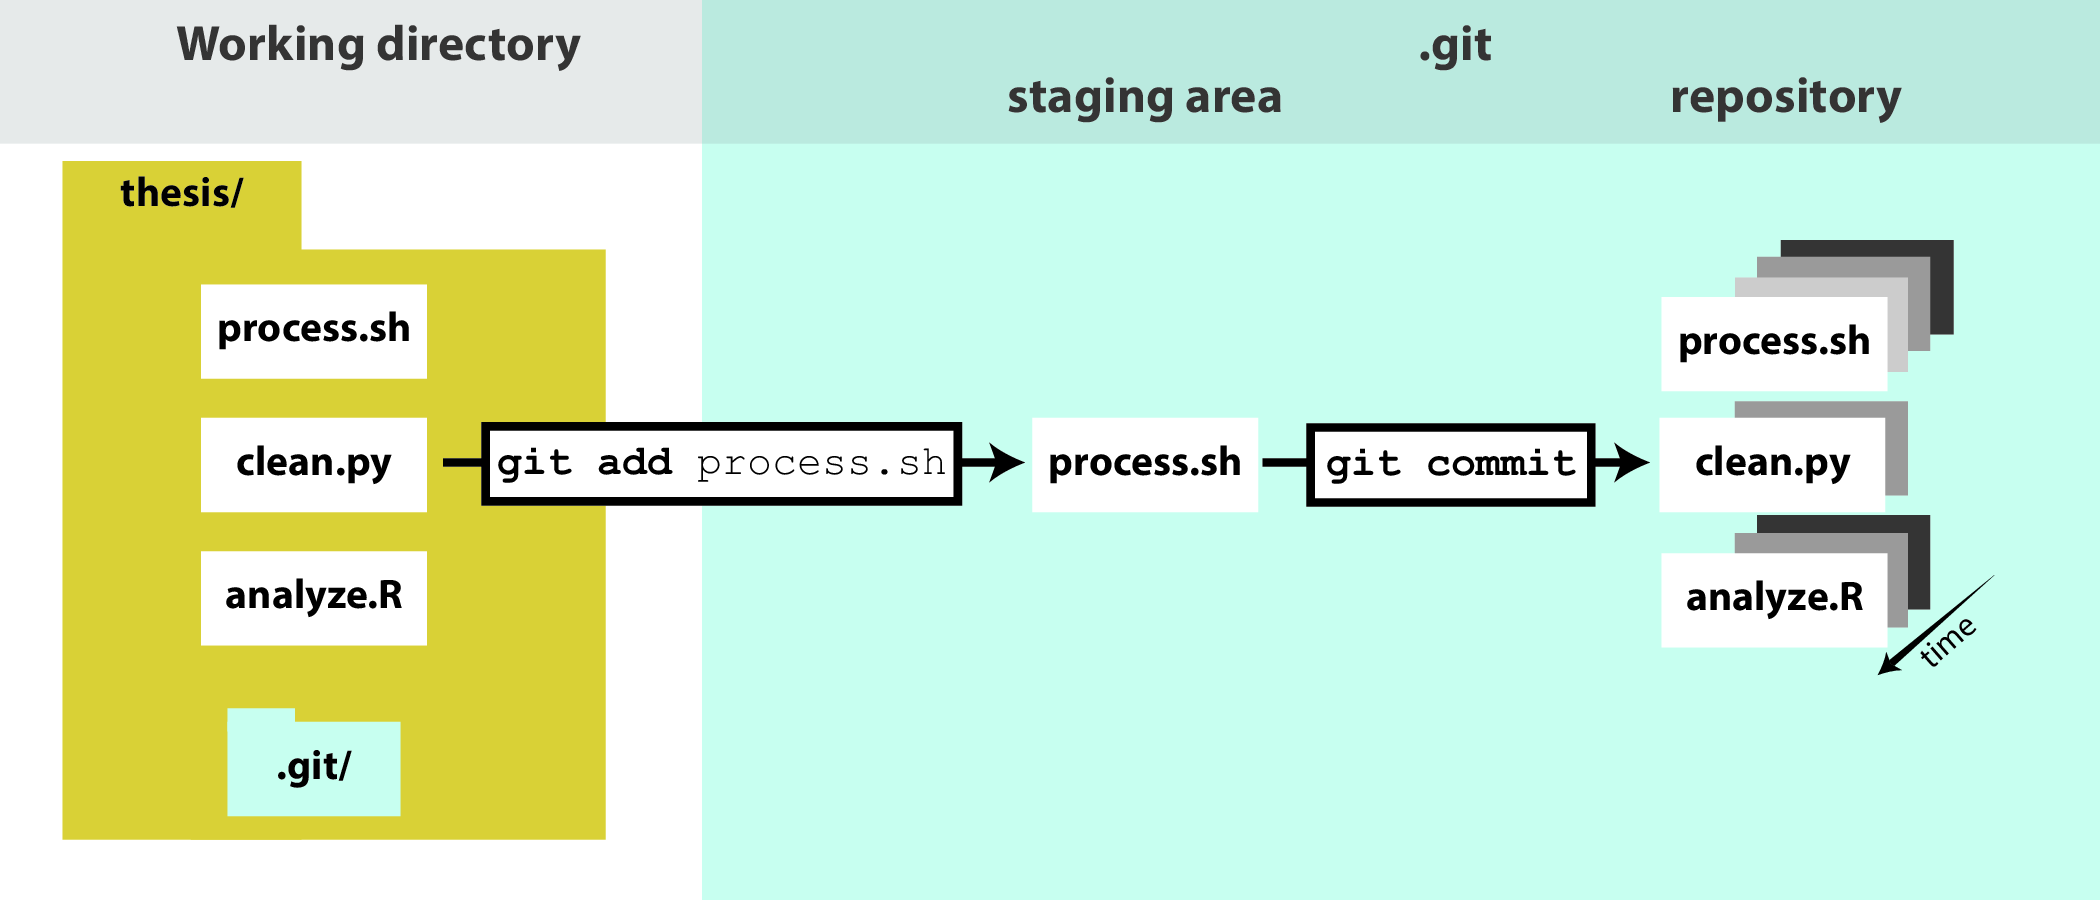
\includegraphics[width=1\columnwidth]{figures/Fig1/Fig1.png}
\caption{\textbf{\label{fig:Fig1}}%
}
\end{center}
\end{figure}

\begin{figure}[h!]
\begin{center}
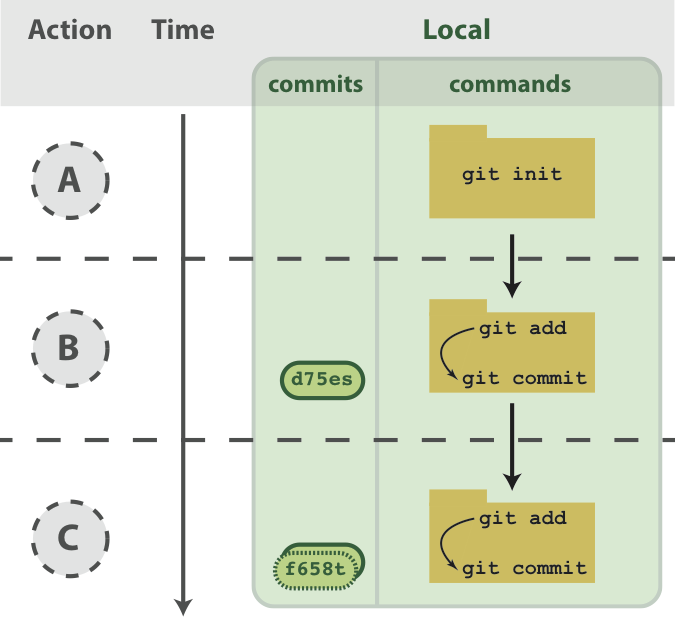
\includegraphics[width=0.7\columnwidth]{figures/Fig2/Fig2.png}
\caption{\textbf{\label{fig:Fig2}}
%
}
\end{center}
\end{figure}

\begin{figure}[h!]
\begin{center}
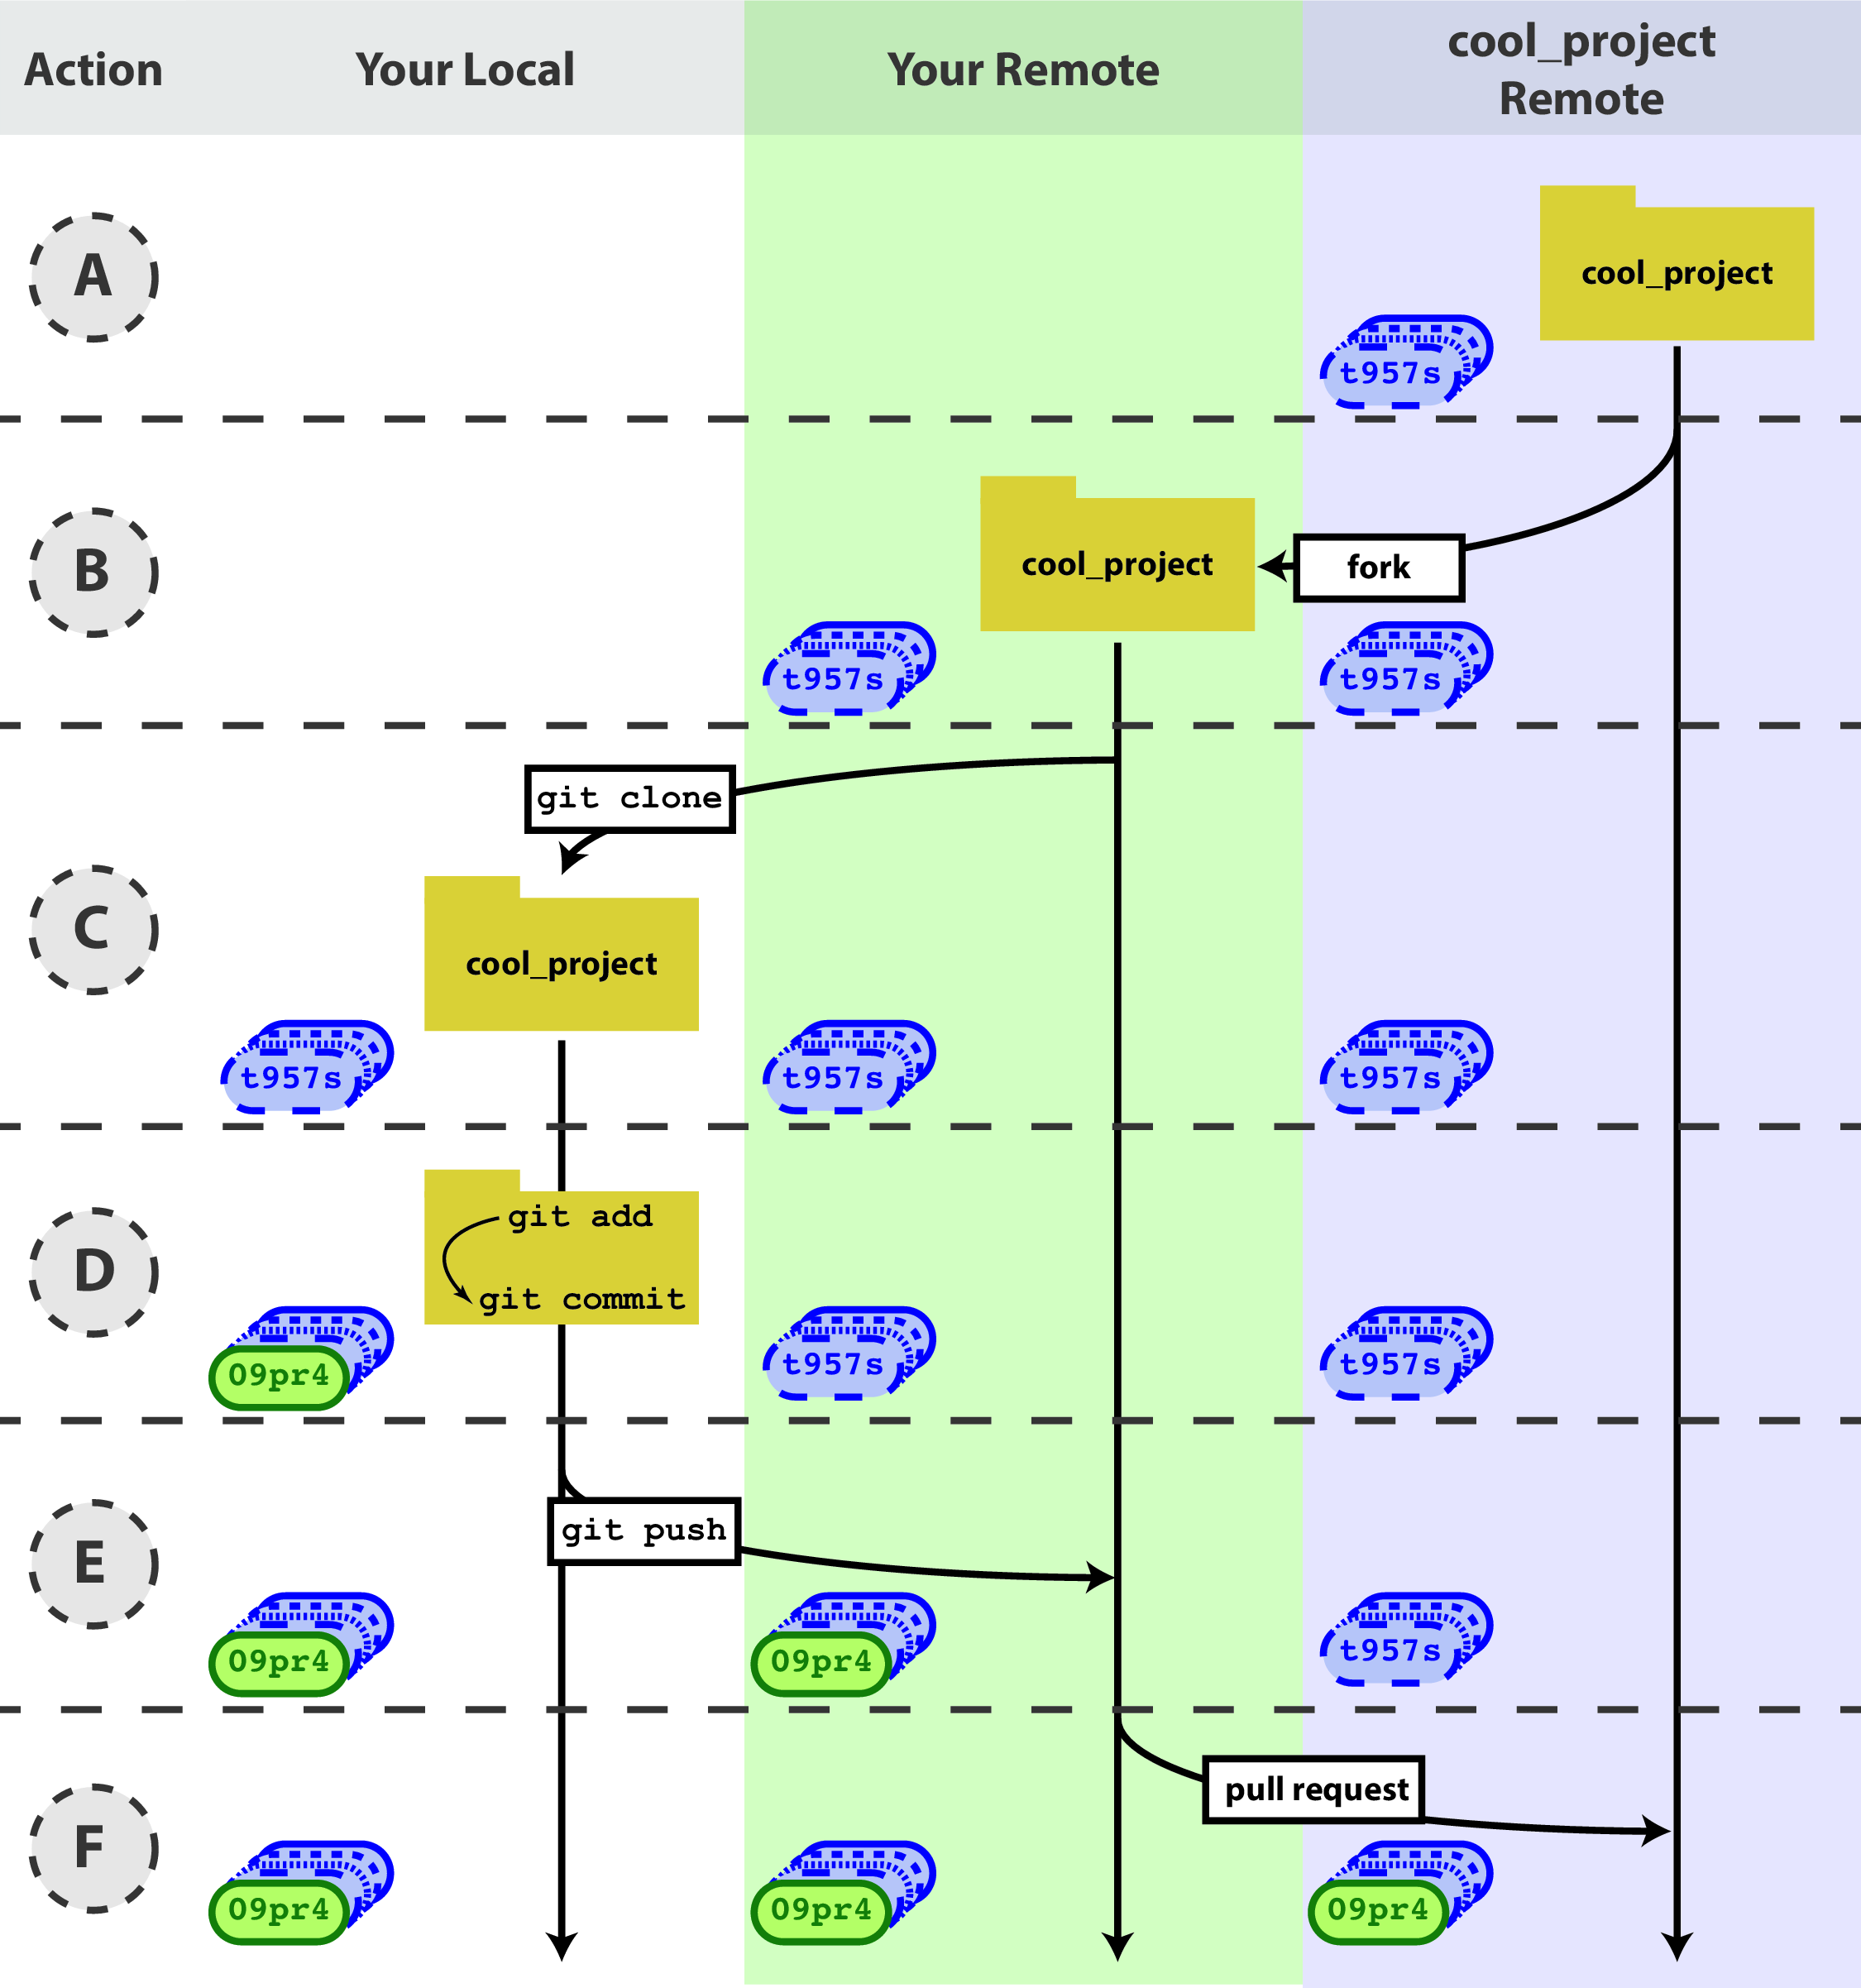
\includegraphics[width=0.7\columnwidth]{figures/Fig3/Fig3.png}
\caption{\textbf{\label{fig:Fig3}}
%
}
\end{center}
\end{figure}

\begin{figure}[h!]
\begin{center}
\DIFdelbeginFL %DIFDELCMD < 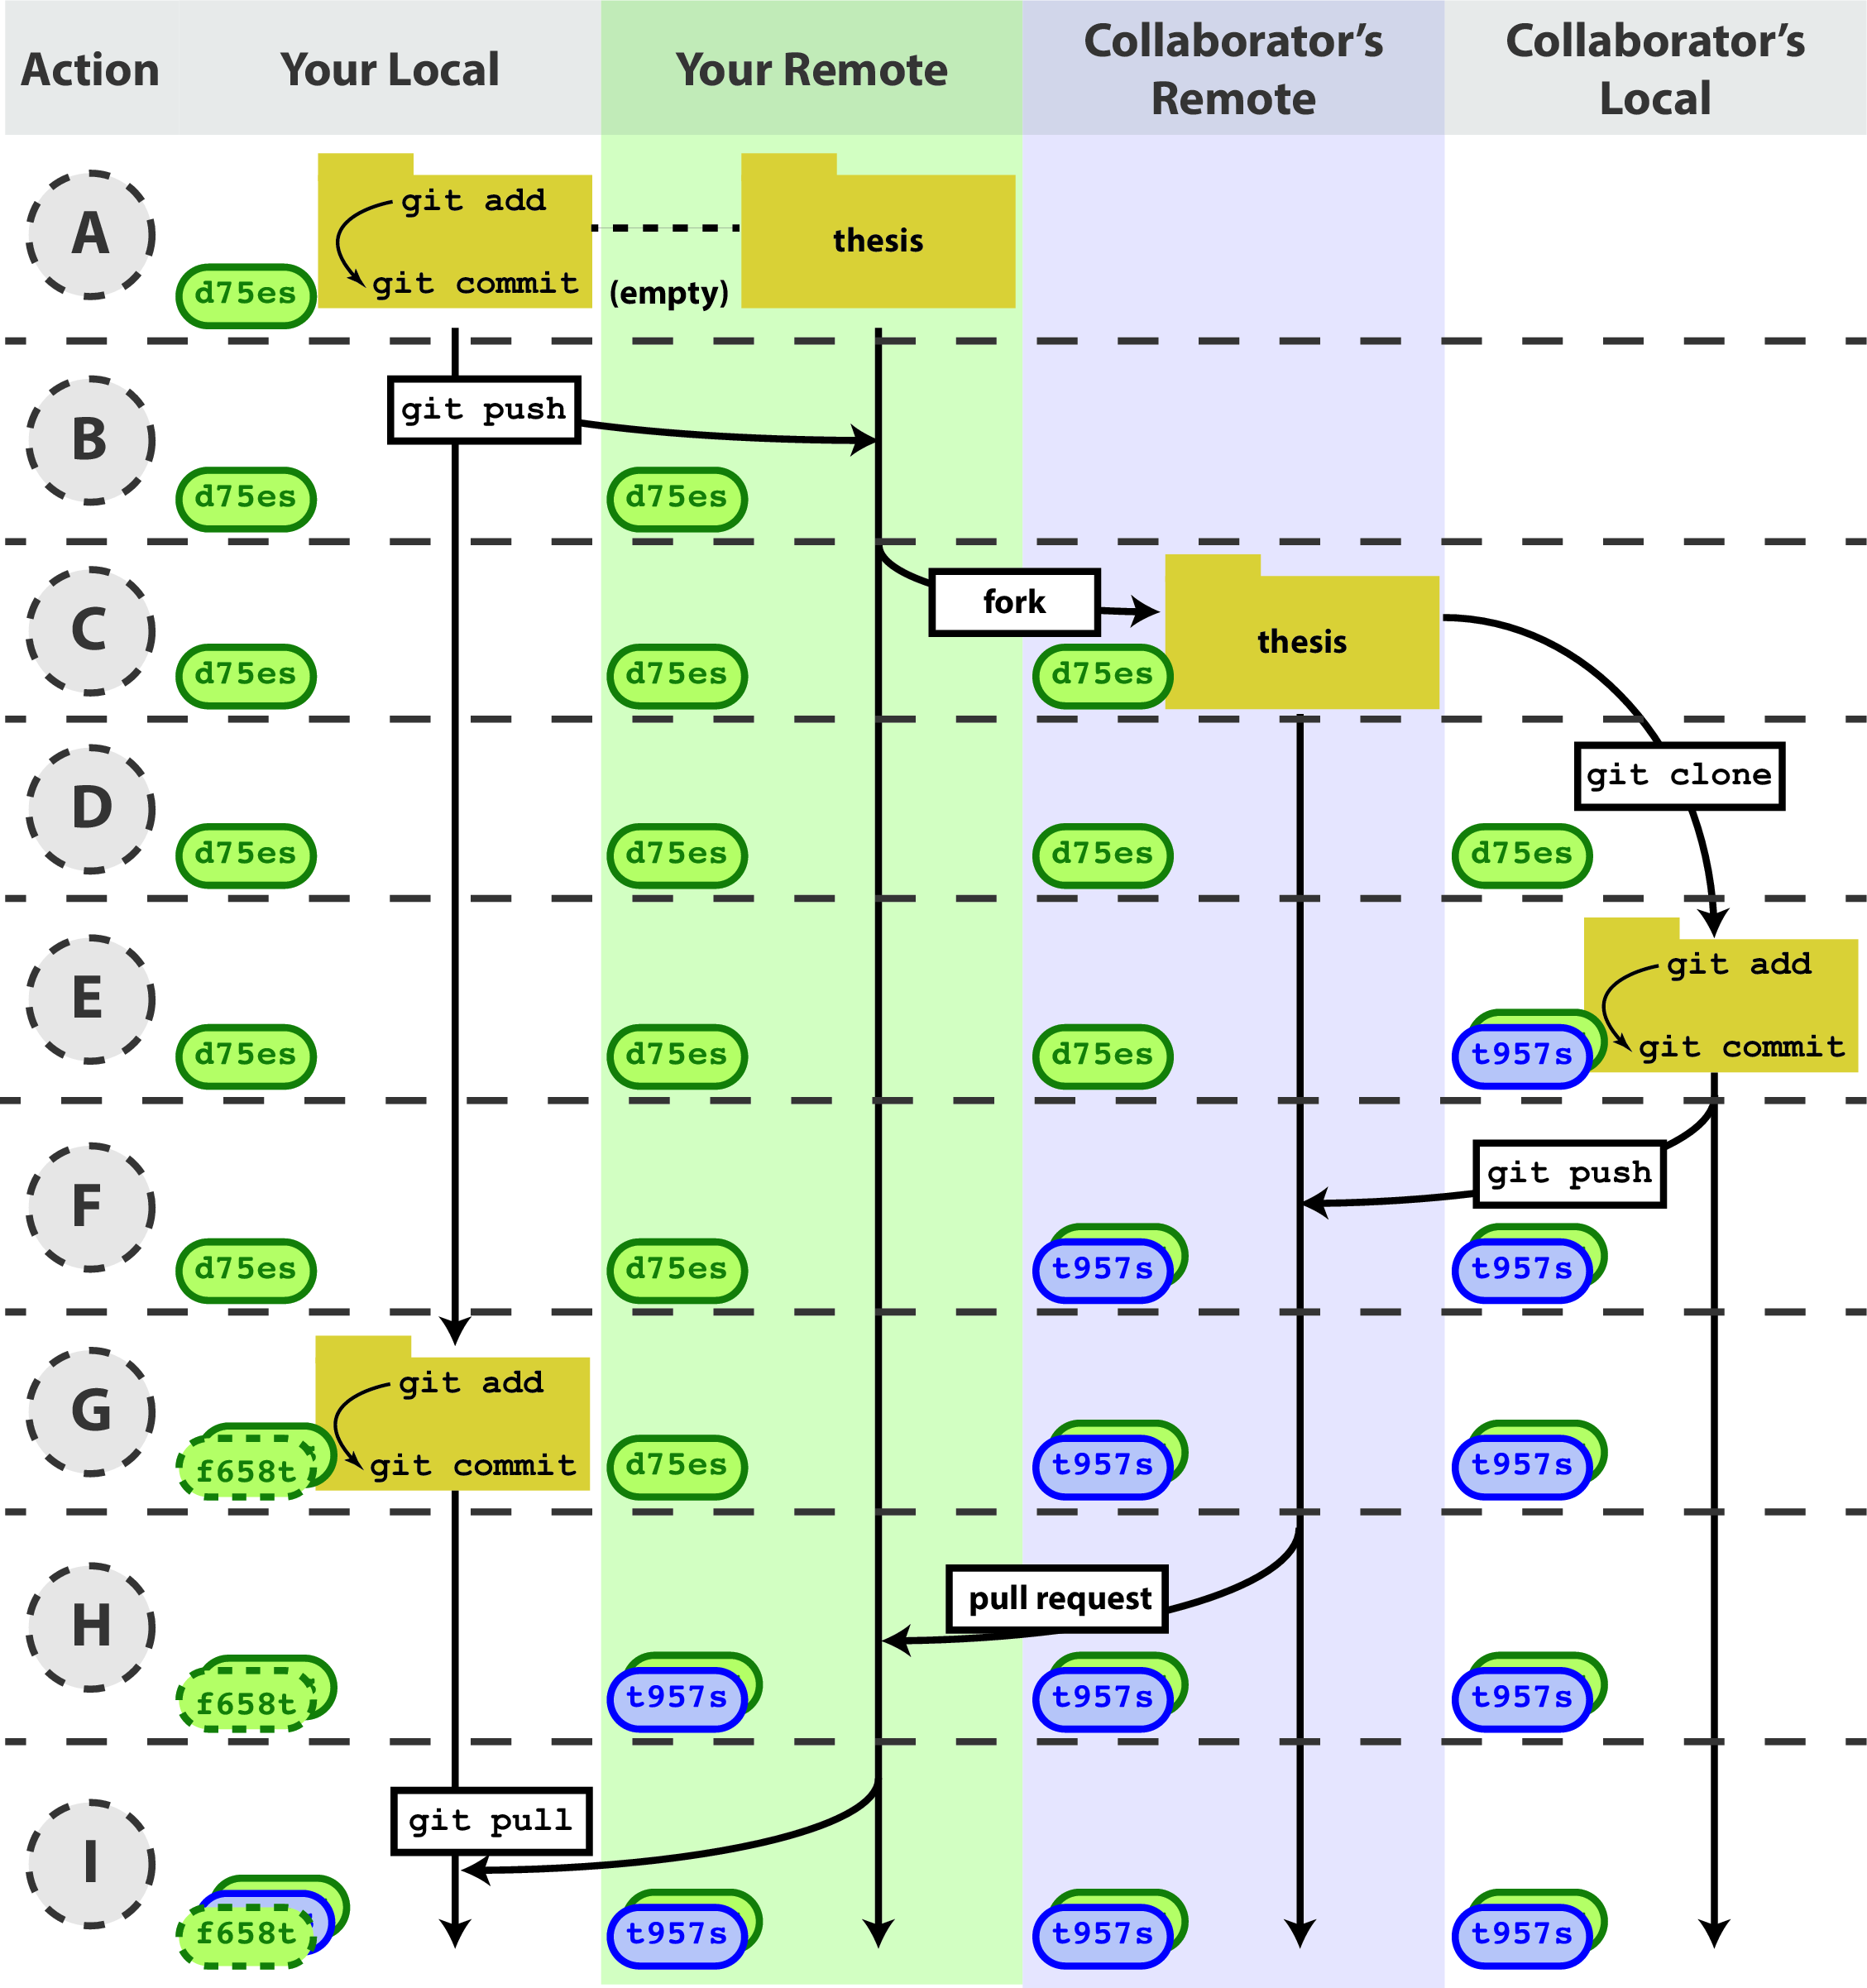
\includegraphics[width=1\columnwidth]{figures/S1_Fig/S1_Fig.png}
%DIFDELCMD < %%%
\DIFdelendFL \DIFaddbeginFL 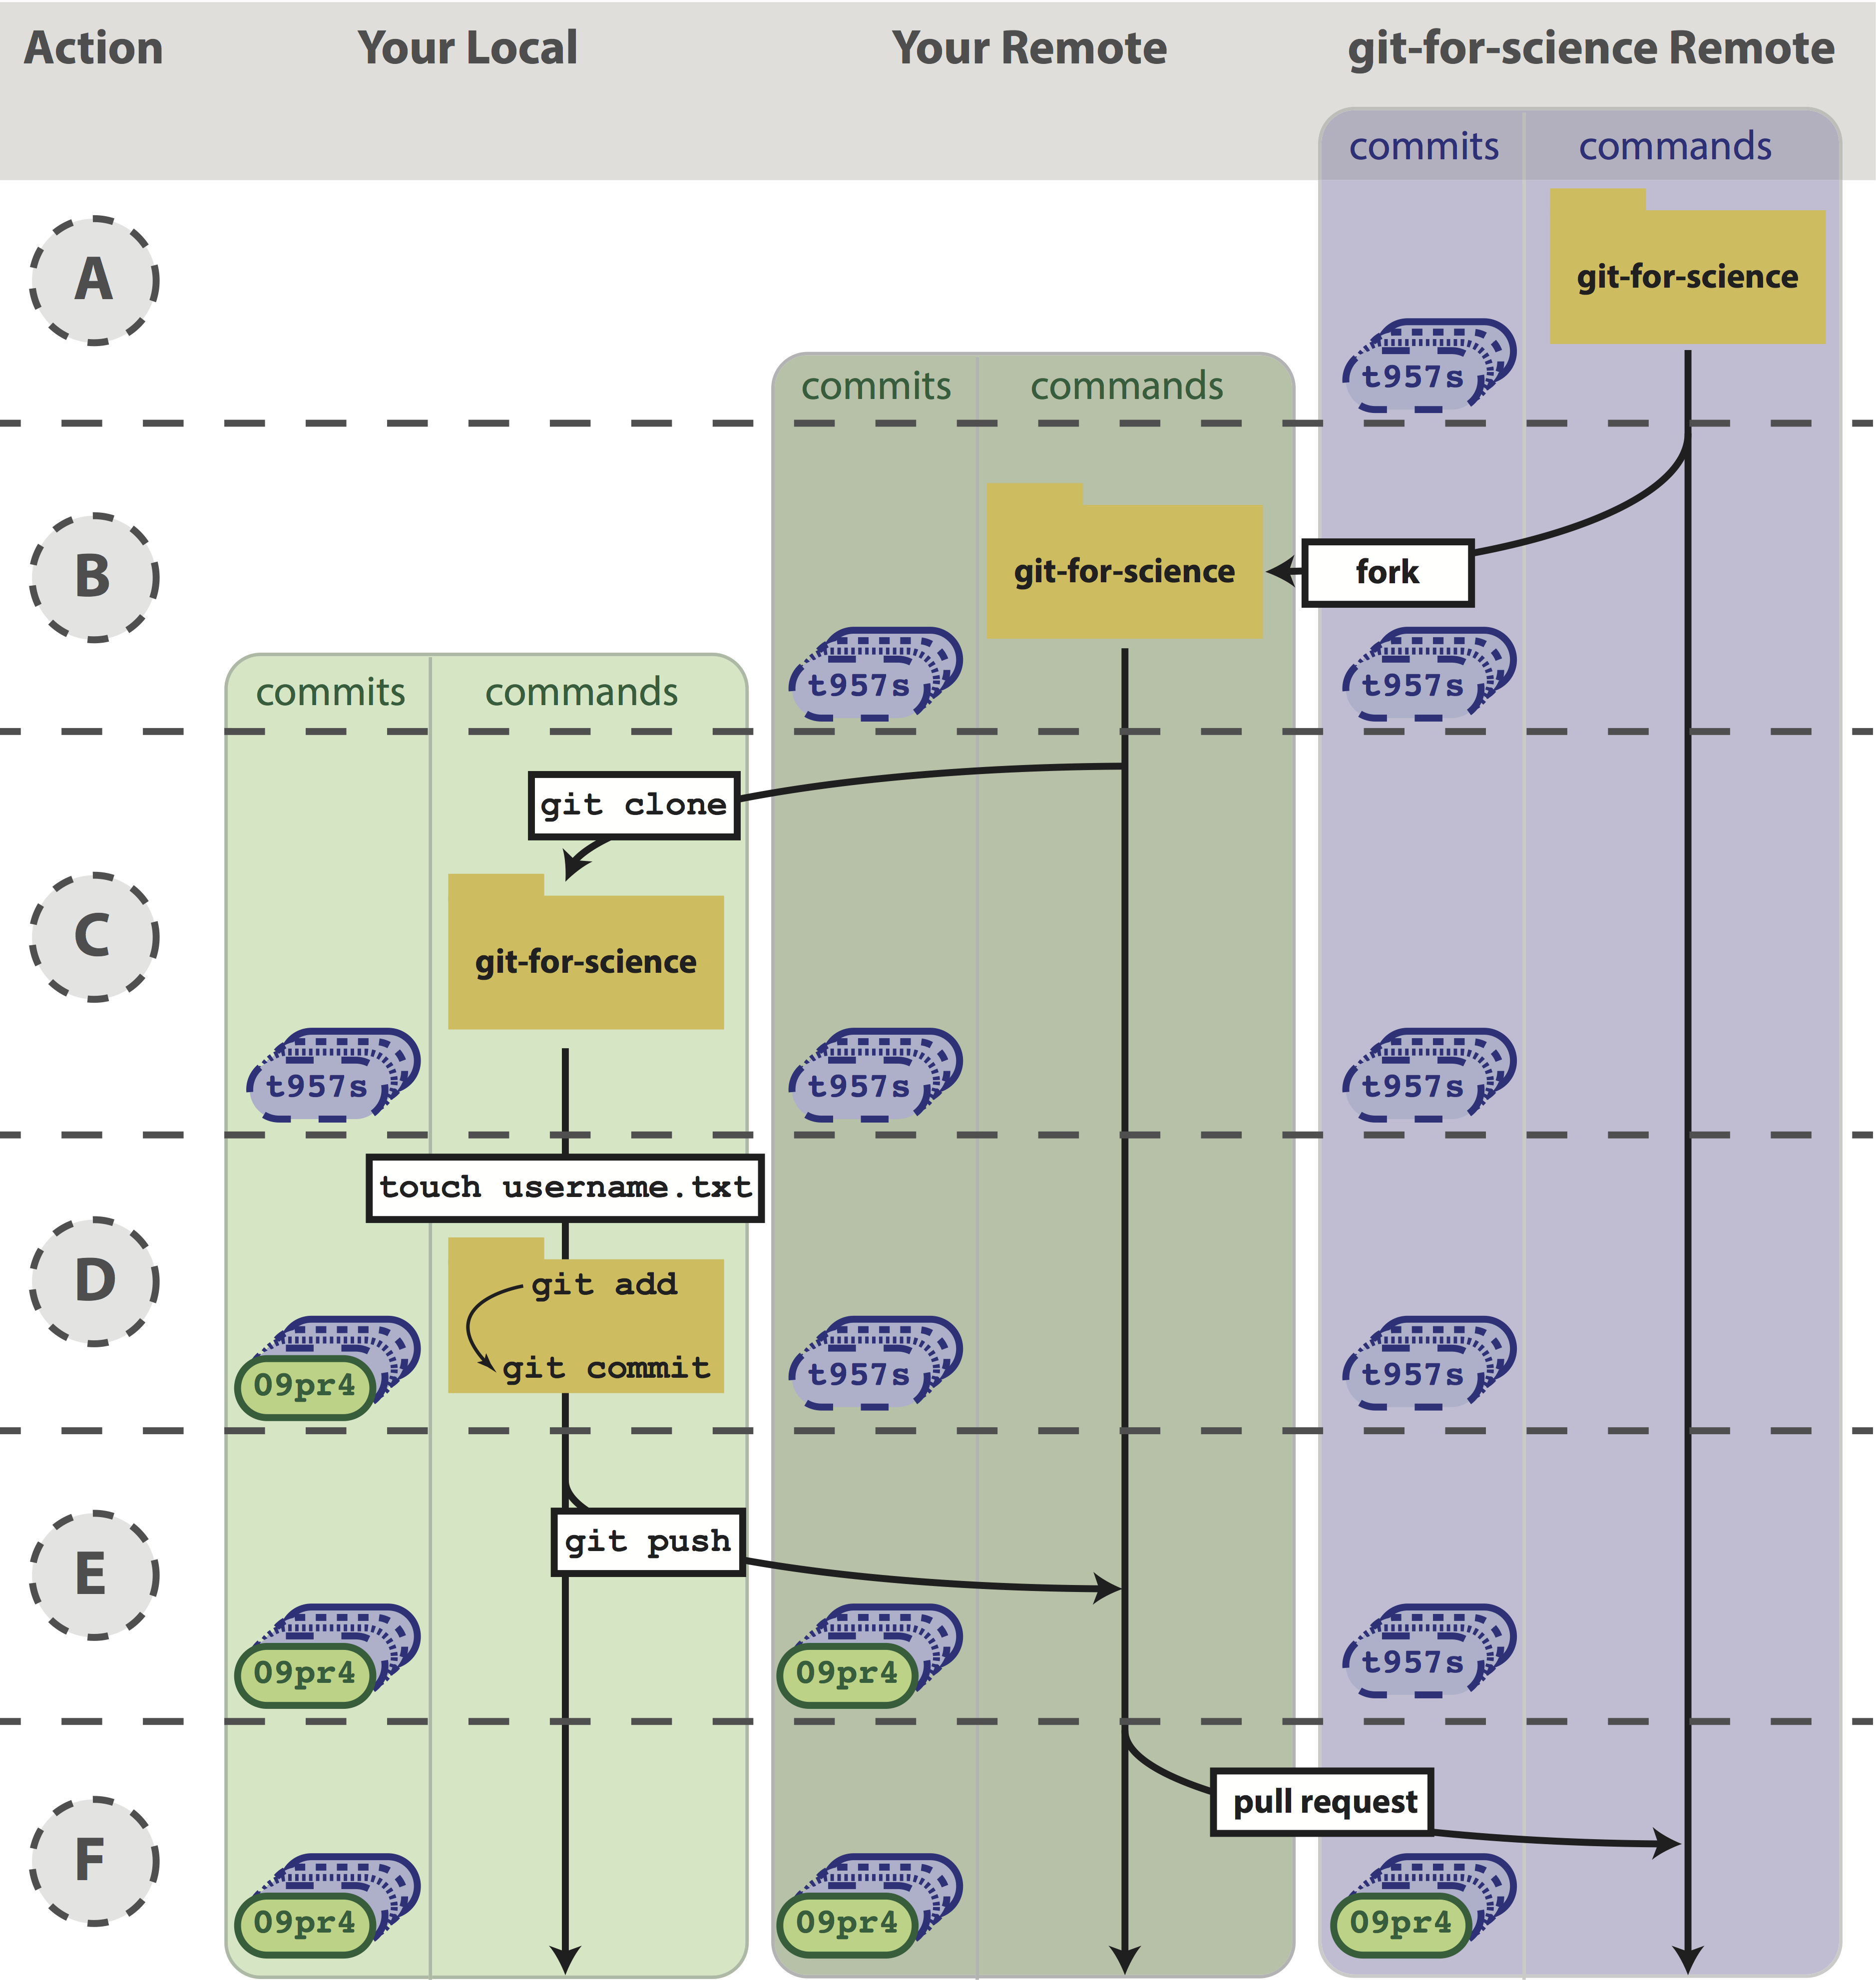
\includegraphics[width=0.7\columnwidth]{figures/Fig4/Fig4.png}
\DIFaddendFL \caption{\DIFdelbeginFL \textbf{%DIFDELCMD < \label{fig:S1_Fig}%%%
}%DIFAUXCMD
\DIFdelendFL \DIFaddbeginFL \textbf{\label{fig:Fig4}}\DIFaddendFL %
}
\end{center}
\end{figure}

\bibliography{bibliography/converted_to_latex.bib%
}

\end{document}

